


% Header, overrides base

    % Make sure that the sphinx doc style knows who it inherits from.
    \def\sphinxdocclass{article}

    % Declare the document class
    \documentclass[letterpaper,10pt,english]{/Users/kinealicegulbrandsen/anaconda/lib/python2.7/site-packages/sphinx/texinputs/sphinxhowto}

    % Imports
    \usepackage[utf8]{inputenc}
    \DeclareUnicodeCharacter{00A0}{\\nobreakspace}
    \usepackage[T1]{fontenc}
    \usepackage{babel}
    \usepackage{times}
    \usepackage{import}
    \usepackage[Bjarne]{/Users/kinealicegulbrandsen/anaconda/lib/python2.7/site-packages/sphinx/texinputs/fncychap}
    \usepackage{longtable}
    \usepackage{/Users/kinealicegulbrandsen/anaconda/lib/python2.7/site-packages/sphinx/texinputs/sphinx}
    \usepackage{multirow}

    \usepackage{amsmath}
    \usepackage{amssymb}
    \usepackage{ucs}
    \usepackage{enumerate}

    % Used to make the Input/Output rules follow around the contents.
    \usepackage{needspace}

    % Pygments requirements
    \usepackage{fancyvrb}
    \usepackage{color}
    % ansi colors additions
    \definecolor{darkgreen}{rgb}{.12,.54,.11}
    \definecolor{lightgray}{gray}{.95}
    \definecolor{brown}{rgb}{0.54,0.27,0.07}
    \definecolor{purple}{rgb}{0.5,0.0,0.5}
    \definecolor{darkgray}{gray}{0.25}
    \definecolor{lightred}{rgb}{1.0,0.39,0.28}
    \definecolor{lightgreen}{rgb}{0.48,0.99,0.0}
    \definecolor{lightblue}{rgb}{0.53,0.81,0.92}
    \definecolor{lightpurple}{rgb}{0.87,0.63,0.87}
    \definecolor{lightcyan}{rgb}{0.5,1.0,0.83}

    % Needed to box output/input
    \usepackage{tikz}
        \usetikzlibrary{calc,arrows,shadows}
    \usepackage[framemethod=tikz]{mdframed}

    \usepackage{alltt}

    % Used to load and display graphics
    \usepackage{graphicx}
    \graphicspath{ {figs/} }
    \usepackage[Export]{adjustbox} % To resize

    % used so that images for notebooks which have spaces in the name can still be included
    \usepackage{grffile}


    % For formatting output while also word wrapping.
    \usepackage{listings}
    \lstset{breaklines=true}
    \lstset{basicstyle=\small\ttfamily}
    \def\smaller{\fontsize{9.5pt}{9.5pt}\selectfont}

    %Pygments definitions
    
\makeatletter
\def\PY@reset{\let\PY@it=\relax \let\PY@bf=\relax%
    \let\PY@ul=\relax \let\PY@tc=\relax%
    \let\PY@bc=\relax \let\PY@ff=\relax}
\def\PY@tok#1{\csname PY@tok@#1\endcsname}
\def\PY@toks#1+{\ifx\relax#1\empty\else%
    \PY@tok{#1}\expandafter\PY@toks\fi}
\def\PY@do#1{\PY@bc{\PY@tc{\PY@ul{%
    \PY@it{\PY@bf{\PY@ff{#1}}}}}}}
\def\PY#1#2{\PY@reset\PY@toks#1+\relax+\PY@do{#2}}

\expandafter\def\csname PY@tok@gd\endcsname{\def\PY@tc##1{\textcolor[rgb]{0.63,0.00,0.00}{##1}}}
\expandafter\def\csname PY@tok@gu\endcsname{\let\PY@bf=\textbf\def\PY@tc##1{\textcolor[rgb]{0.50,0.00,0.50}{##1}}}
\expandafter\def\csname PY@tok@gt\endcsname{\def\PY@tc##1{\textcolor[rgb]{0.00,0.27,0.87}{##1}}}
\expandafter\def\csname PY@tok@gs\endcsname{\let\PY@bf=\textbf}
\expandafter\def\csname PY@tok@gr\endcsname{\def\PY@tc##1{\textcolor[rgb]{1.00,0.00,0.00}{##1}}}
\expandafter\def\csname PY@tok@cm\endcsname{\let\PY@it=\textit\def\PY@tc##1{\textcolor[rgb]{0.25,0.50,0.50}{##1}}}
\expandafter\def\csname PY@tok@vg\endcsname{\def\PY@tc##1{\textcolor[rgb]{0.10,0.09,0.49}{##1}}}
\expandafter\def\csname PY@tok@m\endcsname{\def\PY@tc##1{\textcolor[rgb]{0.40,0.40,0.40}{##1}}}
\expandafter\def\csname PY@tok@mh\endcsname{\def\PY@tc##1{\textcolor[rgb]{0.40,0.40,0.40}{##1}}}
\expandafter\def\csname PY@tok@go\endcsname{\def\PY@tc##1{\textcolor[rgb]{0.53,0.53,0.53}{##1}}}
\expandafter\def\csname PY@tok@ge\endcsname{\let\PY@it=\textit}
\expandafter\def\csname PY@tok@vc\endcsname{\def\PY@tc##1{\textcolor[rgb]{0.10,0.09,0.49}{##1}}}
\expandafter\def\csname PY@tok@il\endcsname{\def\PY@tc##1{\textcolor[rgb]{0.40,0.40,0.40}{##1}}}
\expandafter\def\csname PY@tok@cs\endcsname{\let\PY@it=\textit\def\PY@tc##1{\textcolor[rgb]{0.25,0.50,0.50}{##1}}}
\expandafter\def\csname PY@tok@cp\endcsname{\def\PY@tc##1{\textcolor[rgb]{0.74,0.48,0.00}{##1}}}
\expandafter\def\csname PY@tok@gi\endcsname{\def\PY@tc##1{\textcolor[rgb]{0.00,0.63,0.00}{##1}}}
\expandafter\def\csname PY@tok@gh\endcsname{\let\PY@bf=\textbf\def\PY@tc##1{\textcolor[rgb]{0.00,0.00,0.50}{##1}}}
\expandafter\def\csname PY@tok@ni\endcsname{\let\PY@bf=\textbf\def\PY@tc##1{\textcolor[rgb]{0.60,0.60,0.60}{##1}}}
\expandafter\def\csname PY@tok@nl\endcsname{\def\PY@tc##1{\textcolor[rgb]{0.63,0.63,0.00}{##1}}}
\expandafter\def\csname PY@tok@nn\endcsname{\let\PY@bf=\textbf\def\PY@tc##1{\textcolor[rgb]{0.00,0.00,1.00}{##1}}}
\expandafter\def\csname PY@tok@no\endcsname{\def\PY@tc##1{\textcolor[rgb]{0.53,0.00,0.00}{##1}}}
\expandafter\def\csname PY@tok@na\endcsname{\def\PY@tc##1{\textcolor[rgb]{0.49,0.56,0.16}{##1}}}
\expandafter\def\csname PY@tok@nb\endcsname{\def\PY@tc##1{\textcolor[rgb]{0.00,0.50,0.00}{##1}}}
\expandafter\def\csname PY@tok@nc\endcsname{\let\PY@bf=\textbf\def\PY@tc##1{\textcolor[rgb]{0.00,0.00,1.00}{##1}}}
\expandafter\def\csname PY@tok@nd\endcsname{\def\PY@tc##1{\textcolor[rgb]{0.67,0.13,1.00}{##1}}}
\expandafter\def\csname PY@tok@ne\endcsname{\let\PY@bf=\textbf\def\PY@tc##1{\textcolor[rgb]{0.82,0.25,0.23}{##1}}}
\expandafter\def\csname PY@tok@nf\endcsname{\def\PY@tc##1{\textcolor[rgb]{0.00,0.00,1.00}{##1}}}
\expandafter\def\csname PY@tok@si\endcsname{\let\PY@bf=\textbf\def\PY@tc##1{\textcolor[rgb]{0.73,0.40,0.53}{##1}}}
\expandafter\def\csname PY@tok@s2\endcsname{\def\PY@tc##1{\textcolor[rgb]{0.73,0.13,0.13}{##1}}}
\expandafter\def\csname PY@tok@vi\endcsname{\def\PY@tc##1{\textcolor[rgb]{0.10,0.09,0.49}{##1}}}
\expandafter\def\csname PY@tok@nt\endcsname{\let\PY@bf=\textbf\def\PY@tc##1{\textcolor[rgb]{0.00,0.50,0.00}{##1}}}
\expandafter\def\csname PY@tok@nv\endcsname{\def\PY@tc##1{\textcolor[rgb]{0.10,0.09,0.49}{##1}}}
\expandafter\def\csname PY@tok@s1\endcsname{\def\PY@tc##1{\textcolor[rgb]{0.73,0.13,0.13}{##1}}}
\expandafter\def\csname PY@tok@sh\endcsname{\def\PY@tc##1{\textcolor[rgb]{0.73,0.13,0.13}{##1}}}
\expandafter\def\csname PY@tok@sc\endcsname{\def\PY@tc##1{\textcolor[rgb]{0.73,0.13,0.13}{##1}}}
\expandafter\def\csname PY@tok@sx\endcsname{\def\PY@tc##1{\textcolor[rgb]{0.00,0.50,0.00}{##1}}}
\expandafter\def\csname PY@tok@bp\endcsname{\def\PY@tc##1{\textcolor[rgb]{0.00,0.50,0.00}{##1}}}
\expandafter\def\csname PY@tok@c1\endcsname{\let\PY@it=\textit\def\PY@tc##1{\textcolor[rgb]{0.25,0.50,0.50}{##1}}}
\expandafter\def\csname PY@tok@kc\endcsname{\let\PY@bf=\textbf\def\PY@tc##1{\textcolor[rgb]{0.00,0.50,0.00}{##1}}}
\expandafter\def\csname PY@tok@c\endcsname{\let\PY@it=\textit\def\PY@tc##1{\textcolor[rgb]{0.25,0.50,0.50}{##1}}}
\expandafter\def\csname PY@tok@mf\endcsname{\def\PY@tc##1{\textcolor[rgb]{0.40,0.40,0.40}{##1}}}
\expandafter\def\csname PY@tok@err\endcsname{\def\PY@bc##1{\setlength{\fboxsep}{0pt}\fcolorbox[rgb]{1.00,0.00,0.00}{1,1,1}{\strut ##1}}}
\expandafter\def\csname PY@tok@kd\endcsname{\let\PY@bf=\textbf\def\PY@tc##1{\textcolor[rgb]{0.00,0.50,0.00}{##1}}}
\expandafter\def\csname PY@tok@ss\endcsname{\def\PY@tc##1{\textcolor[rgb]{0.10,0.09,0.49}{##1}}}
\expandafter\def\csname PY@tok@sr\endcsname{\def\PY@tc##1{\textcolor[rgb]{0.73,0.40,0.53}{##1}}}
\expandafter\def\csname PY@tok@mo\endcsname{\def\PY@tc##1{\textcolor[rgb]{0.40,0.40,0.40}{##1}}}
\expandafter\def\csname PY@tok@kn\endcsname{\let\PY@bf=\textbf\def\PY@tc##1{\textcolor[rgb]{0.00,0.50,0.00}{##1}}}
\expandafter\def\csname PY@tok@mi\endcsname{\def\PY@tc##1{\textcolor[rgb]{0.40,0.40,0.40}{##1}}}
\expandafter\def\csname PY@tok@gp\endcsname{\let\PY@bf=\textbf\def\PY@tc##1{\textcolor[rgb]{0.00,0.00,0.50}{##1}}}
\expandafter\def\csname PY@tok@o\endcsname{\def\PY@tc##1{\textcolor[rgb]{0.40,0.40,0.40}{##1}}}
\expandafter\def\csname PY@tok@kr\endcsname{\let\PY@bf=\textbf\def\PY@tc##1{\textcolor[rgb]{0.00,0.50,0.00}{##1}}}
\expandafter\def\csname PY@tok@s\endcsname{\def\PY@tc##1{\textcolor[rgb]{0.73,0.13,0.13}{##1}}}
\expandafter\def\csname PY@tok@kp\endcsname{\def\PY@tc##1{\textcolor[rgb]{0.00,0.50,0.00}{##1}}}
\expandafter\def\csname PY@tok@w\endcsname{\def\PY@tc##1{\textcolor[rgb]{0.73,0.73,0.73}{##1}}}
\expandafter\def\csname PY@tok@kt\endcsname{\def\PY@tc##1{\textcolor[rgb]{0.69,0.00,0.25}{##1}}}
\expandafter\def\csname PY@tok@ow\endcsname{\let\PY@bf=\textbf\def\PY@tc##1{\textcolor[rgb]{0.67,0.13,1.00}{##1}}}
\expandafter\def\csname PY@tok@sb\endcsname{\def\PY@tc##1{\textcolor[rgb]{0.73,0.13,0.13}{##1}}}
\expandafter\def\csname PY@tok@k\endcsname{\let\PY@bf=\textbf\def\PY@tc##1{\textcolor[rgb]{0.00,0.50,0.00}{##1}}}
\expandafter\def\csname PY@tok@se\endcsname{\let\PY@bf=\textbf\def\PY@tc##1{\textcolor[rgb]{0.73,0.40,0.13}{##1}}}
\expandafter\def\csname PY@tok@sd\endcsname{\let\PY@it=\textit\def\PY@tc##1{\textcolor[rgb]{0.73,0.13,0.13}{##1}}}

\def\PYZbs{\char`\\}
\def\PYZus{\char`\_}
\def\PYZob{\char`\{}
\def\PYZcb{\char`\}}
\def\PYZca{\char`\^}
\def\PYZam{\char`\&}
\def\PYZlt{\char`\<}
\def\PYZgt{\char`\>}
\def\PYZsh{\char`\#}
\def\PYZpc{\char`\%}
\def\PYZdl{\char`\$}
\def\PYZhy{\char`\-}
\def\PYZsq{\char`\'}
\def\PYZdq{\char`\"}
\def\PYZti{\char`\~}
% for compatibility with earlier versions
\def\PYZat{@}
\def\PYZlb{[}
\def\PYZrb{]}
\makeatother


    %Set pygments styles if needed...
    
        \definecolor{nbframe-border}{rgb}{0.867,0.867,0.867}
        \definecolor{nbframe-bg}{rgb}{0.969,0.969,0.969}
        \definecolor{nbframe-in-prompt}{rgb}{0.0,0.0,0.502}
        \definecolor{nbframe-out-prompt}{rgb}{0.545,0.0,0.0}

        \newenvironment{ColorVerbatim}
        {\begin{mdframed}[%
            roundcorner=1.0pt, %
            backgroundcolor=nbframe-bg, %
            userdefinedwidth=1\linewidth, %
            leftmargin=0.1\linewidth, %
            innerleftmargin=0pt, %
            innerrightmargin=0pt, %
            linecolor=nbframe-border, %
            linewidth=1pt, %
            usetwoside=false, %
            everyline=true, %
            innerlinewidth=3pt, %
            innerlinecolor=nbframe-bg, %
            middlelinewidth=1pt, %
            middlelinecolor=nbframe-bg, %
            outerlinewidth=0.5pt, %
            outerlinecolor=nbframe-border, %
            needspace=0pt
        ]}
        {\end{mdframed}}
        
        \newenvironment{InvisibleVerbatim}
        {\begin{mdframed}[leftmargin=0.1\linewidth,innerleftmargin=3pt,innerrightmargin=3pt, userdefinedwidth=1\linewidth, linewidth=0pt, linecolor=white, usetwoside=false]}
        {\end{mdframed}}

        \renewenvironment{Verbatim}[1][\unskip]
        {\begin{alltt}\smaller}
        {\end{alltt}}
    

    % Help prevent overflowing lines due to urls and other hard-to-break 
    % entities.  This doesn't catch everything...
    \sloppy

    % Document level variables
    \title{ccalgebra\_for\_web}
    \date{April 11, 2015}
    \release{}
    \author{Unknown Author}
    \renewcommand{\releasename}{}

    % TODO: Add option for the user to specify a logo for his/her export.
    \newcommand{\sphinxlogo}{}

    % Make the index page of the document.
    \makeindex

    % Import sphinx document type specifics.
     


% Body

    % Start of the document
    \begin{document}

        
            \maketitle
        

        


        
        \section{Instructions on using this
notebook}\label{instructions-on-using-this-notebook}

Replace the working directory below with the one you have
CCAlgebra\_mk4.py located.

    % Make sure that atleast 4 lines are below the HR
    \needspace{4\baselineskip}

    
        \vspace{6pt}
        \makebox[0.1\linewidth]{\smaller\hfill\tt\color{nbframe-in-prompt}In\hspace{4pt}{[}3{]}:\hspace{4pt}}\\*
        \vspace{-2.65\baselineskip}
        \begin{ColorVerbatim}
            \vspace{-0.7\baselineskip}
            \begin{Verbatim}[commandchars=\\\{\}]
\PY{k+kn}{from} \PY{n+nn}{IPython.display} \PY{k+kn}{import} \PY{n}{display}\PY{p}{,} \PY{n}{Math}\PY{p}{,} \PY{n}{Latex} 
\PY{o}{\PYZpc{}}\PY{k}{matplotlib} \PY{n}{inline}  
\PY{o}{\PYZpc{}}\PY{k}{cd} \PY{l+s}{\PYZsq{}}\PY{l+s}{\PYZsq{}} \PY{c}{\PYZsh{}insert full path here}
\PY{o}{\PYZpc{}}\PY{k}{run} \PY{n}{CCAlgebra\PYZus{}mk4}\PY{o}{.}\PY{n}{py}
\end{Verbatim}

            
                \vspace{-0.2\baselineskip}
            
        \end{ColorVerbatim}
    
\subsection{Coupled Cluster Diagrammatic
Algebra}\label{coupled-cluster-diagrammatic-algebra}

\paragraph{A python script for learning and developing code for CC
calculations}\label{a-python-script-for-learning-and-developing-code-for-cc-calculations}

\paragraph{Audun Skau Hansen \textbar{} Comp-Phys \textbar{} UiO
\textbar{} 2015}\label{audun-skau-hansen-comp-phys-uio-2015}

\emph{``Because of the often large number of terms in all versions of
the CCM it is rather hard work to obtain the explicit equations by hand.
And after this is done one has to write a program to put them into the
computer.''} - H. G. Kümmel

The code imported in this notebook is intended to provide an environment
for deriving CC equations, complementary code and diagrams using the
diagrammatic approach outlined in Shavitt and Bartlett (S-B) (p.~292).
The code is mainly written for educational purposes, and has not been
extensively tested, optimized or cleaned.

The core operation in CCAlgebra is to extract diagrams from contractions
of operators. A lot of physicists in the field of many body quantum
mechanics appreciate the simplicity and richness of working with
diagrammatic rules alongside second quantization. This code is an
attempt to translate these diagrammatic rules into operations
understandable by the computer, so we may utilize these rules to
generate the full complexity of CC equations of any truncation, for very
general normal ordered hamiltonians. (All operators defined in this code
is assumed to be normal ordered - this is explained in more detail
below. )

The following series of examples is meant to illustrate some of the
potential of the code, and at the same time function as a tutorial for
anyone who wish to use it to derive other equations or diagrams. A
fundamental understanding of second quantization, diagrams and the CC
method is a prerequisite.

I hope to continue the developement of this code after I hand in my
thesis this summer.\subsubsection{1. Defining operators -
Operator()}\label{defining-operators---operator}

The operators we work with here are the cluster operators (T\_1, T\_2
\ldots{}) and the hamiltonian operators. Normal ordering of the
hamiltonian for a system of interacting particles will typically produce
a number of parts, each corresponding to a diagrammatic filament. This
is discussed in more detail in S-B (p.~112, 4.29). \emph{(By filament, I
mean a single, unconnected operator, that in itself would not produce
any contribution when evaluated on the vacuum state.)}

In CCalgebra operators are defined as shown below. The hamiltonian
filament given here corresponds to the last diagram on page 180 in S-B,
(9.105).

    % Make sure that atleast 4 lines are below the HR
    \needspace{4\baselineskip}

    
        \vspace{6pt}
        \makebox[0.1\linewidth]{\smaller\hfill\tt\color{nbframe-in-prompt}In\hspace{4pt}{[}3{]}:\hspace{4pt}}\\*
        \vspace{-2.65\baselineskip}
        \begin{ColorVerbatim}
            \vspace{-0.7\baselineskip}
            \begin{Verbatim}[commandchars=\\\{\}]
\PY{c}{\PYZsh{}How to define operators}
\PY{n}{H}   \PY{o}{=} \PY{n}{Operator}\PY{p}{(}\PY{p}{[}\PY{l+m+mi}{1}\PY{p}{,}\PY{o}{\PYZhy{}}\PY{l+m+mi}{1}\PY{p}{]}\PY{p}{,}\PY{p}{[}\PY{p}{]}\PY{p}{)}      \PY{c}{\PYZsh{} The first list defines q\PYZhy{}particle annihilations (below interaction),}
                               \PY{c}{\PYZsh{} while the second is creations. Particles and holes are indicated by 1 and \PYZhy{}1 respectively.}
    
\PY{n}{T\PYZus{}1} \PY{o}{=} \PY{n}{Operator}\PY{p}{(}\PY{p}{[}\PY{p}{]}\PY{p}{,}\PY{p}{[}\PY{l+m+mi}{1}\PY{p}{,}\PY{o}{\PYZhy{}}\PY{l+m+mi}{1}\PY{p}{]}\PY{p}{)}      \PY{c}{\PYZsh{}The T\PYZus{}1 cluster operator}
\PY{n}{T\PYZus{}2} \PY{o}{=} \PY{n}{Operator}\PY{p}{(}\PY{p}{[}\PY{p}{]}\PY{p}{,}\PY{p}{[}\PY{l+m+mi}{1}\PY{p}{,}\PY{l+m+mi}{1}\PY{p}{,}\PY{o}{\PYZhy{}}\PY{l+m+mi}{1}\PY{p}{,}\PY{o}{\PYZhy{}}\PY{l+m+mi}{1}\PY{p}{]}\PY{p}{)} \PY{c}{\PYZsh{}The T\PYZus{}2 operator; all lists must be normal ordered}
\end{Verbatim}

            
                \vspace{-0.2\baselineskip}
            
        \end{ColorVerbatim}
    
Note that the q-particle operators are given in normal order -
q-particle creation operators to the left.\subsubsection{2. Connecting operators -
O()}\label{connecting-operators---o}

Operators may be diagrammatically connected by applying the rules laid
out in S-B (p.298-299). The implementation in CCAlgebra uses the
permutations library of python to produce all possible ways of
connecting the diagrams, whereby it sorts out the distinct diagrams.

The basic rules are that all lines below the hamiltonian filament must
connect to the one of the cluster operators, and all cluster operators
must be connected to the hamiltonian filament. When this connection of
operators acts on the vacuum state, it may produce an excitation or it
may leave the vacuum state at the same energy level.

A class object O(O1, {[}O2, O3, \ldots{}{]}) is defined and will contain
all distinct ways of connecting the operators. (The name should probably
be changed to something more explanatory such as ``connections()''. An
example is given by connecting the previously defined operators:

    % Make sure that atleast 4 lines are below the HR
    \needspace{4\baselineskip}

    
        \vspace{6pt}
        \makebox[0.1\linewidth]{\smaller\hfill\tt\color{nbframe-in-prompt}In\hspace{4pt}{[}4{]}:\hspace{4pt}}\\*
        \vspace{-2.65\baselineskip}
        \begin{ColorVerbatim}
            \vspace{-0.7\baselineskip}
            \begin{Verbatim}[commandchars=\\\{\}]
\PY{n}{contraction} \PY{o}{=} \PY{n}{O}\PY{p}{(}\PY{n}{H}\PY{p}{,}\PY{p}{[}\PY{n}{T\PYZus{}1}\PY{p}{]}\PY{p}{)} \PY{c}{\PYZsh{}The second argument must be a list of operators (T\PYZus{}1 * T\PYZus{}1 = [T\PYZus{}1, T\PYZus{}1])}
\end{Verbatim}

            
                \vspace{-0.2\baselineskip}
            
        \end{ColorVerbatim}
    
\subsubsection{3. Display and interpret
results}\label{display-and-interpret-results}

All results may be displayed as (1) latex, (2) diagrams (3) a piece of
(``naïve'') C++ code, or simply (4) a report of how the contraction was
interpreted by O(). This last functionality is meant to assist in the
debugging process.\subsubsection{3.1 Excitation level and number of
diagrams}\label{excitation-level-and-number-of-diagrams}

A connection of operators will in principle produce a new set of
operators, which share a common property understood as the excitation
level of the operators. Any operator in second quantization have this
property, and it is easily evaluated by counting the number of lines
exiting the operator and subtracting the the number of lines entering
the operator. The excitation level is this number divided by 2, as the
interaction should leave the number of particles constant.

Considering the connection made above, we may evaluate the excitation
level as well as the number of distinct diagrams produced in the
connection:

    % Make sure that atleast 4 lines are below the HR
    \needspace{4\baselineskip}

    
        \vspace{6pt}
        \makebox[0.1\linewidth]{\smaller\hfill\tt\color{nbframe-in-prompt}In\hspace{4pt}{[}4{]}:\hspace{4pt}}\\*
        \vspace{-2.65\baselineskip}
        \begin{ColorVerbatim}
            \vspace{-0.7\baselineskip}
            \begin{Verbatim}[commandchars=\\\{\}]
\PY{k}{print} \PY{l+s}{\PYZdq{}}\PY{l+s}{Excitation:}\PY{l+s}{\PYZdq{}}\PY{p}{,} \PY{n}{contraction}\PY{o}{.}\PY{n}{E}\PY{p}{(}\PY{p}{)} \PY{c}{\PYZsh{}Excitation energy of connected operators}
\PY{k}{print} \PY{l+s}{\PYZdq{}}\PY{l+s}{Number of distinct diagrams:}\PY{l+s}{\PYZdq{}}\PY{p}{,} \PY{n}{contraction}\PY{o}{.}\PY{n}{N}
\end{Verbatim}

            
                \vspace{-0.2\baselineskip}
            
        \end{ColorVerbatim}
    

    

        % If the first block is an image, minipage the image.  Else
        % request a certain amount of space for the input text.
        \needspace{4\baselineskip}
        
        

            % Add document contents.
            
                \begin{InvisibleVerbatim}
                \vspace{-0.5\baselineskip}
\begin{alltt}Excitation: 0.0
Number of distinct diagrams: 1
\end{alltt}

            \end{InvisibleVerbatim}
            
        
    
\subsubsection{3.2 Mathematical
representation}\label{mathematical-representation}

We may then interpret the 0th (the only) connection produced as a latex
formatted string:

    % Make sure that atleast 4 lines are below the HR
    \needspace{4\baselineskip}

    
        \vspace{6pt}
        \makebox[0.1\linewidth]{\smaller\hfill\tt\color{nbframe-in-prompt}In\hspace{4pt}{[}5{]}:\hspace{4pt}}\\*
        \vspace{-2.65\baselineskip}
        \begin{ColorVerbatim}
            \vspace{-0.7\baselineskip}
            \begin{Verbatim}[commandchars=\\\{\}]
\PY{n}{c\PYZus{}tex} \PY{o}{=} \PY{n}{contraction}\PY{o}{.}\PY{n}{latex}\PY{p}{(}\PY{l+m+mi}{0}\PY{p}{)} \PY{c}{\PYZsh{}The first of possibly multiple distinct diagrams in latex format.}
\PY{n}{Math}\PY{p}{(}\PY{n}{c\PYZus{}tex}\PY{p}{)}
\end{Verbatim}

            
                \vspace{-0.2\baselineskip}
            
        \end{ColorVerbatim}
    

    

        % If the first block is an image, minipage the image.  Else
        % request a certain amount of space for the input text.
        \needspace{4\baselineskip}
        
        

            % Add document contents.
            
                \makebox[0.1\linewidth]{\smaller\hfill\tt\color{nbframe-out-prompt}Out\hspace{4pt}{[}5{]}:\hspace{4pt}}\\*
                \vspace{-2.55\baselineskip}\begin{InvisibleVerbatim}
                \vspace{-0.5\baselineskip}
$$\frac{1}{1} \sum_{ck} \langle k || c \rangle t_{k}^{c}$$
            \end{InvisibleVerbatim}
            
        
    
Compare this sum to the middle upper diagram on page 297 in S-B. As the
final excitation of this diagram is 0, it will contribute to the energy
equation. Note that while S-B makes an exception in the labelling of
internal lines in the energy diagrams, CCAlgebra does not make this
distinction. (S-B reserves the labels \emph{a,b,i,j} for target indices
in general, except for the energy contribution.)

\textbf{Note:} It is unfortunate to use the ``double vertical bar''
(antisymmetric) notation for the single particle energy as in the case
above. This is one of many minor details that will be corrected in later
versions of the code.\subsubsection{3.3 Diagrammatic
representation}\label{diagrammatic-representation}

To compare the sum to its diagrammatic counterpart, we write:

    % Make sure that atleast 4 lines are below the HR
    \needspace{4\baselineskip}

    
        \vspace{6pt}
        \makebox[0.1\linewidth]{\smaller\hfill\tt\color{nbframe-in-prompt}In\hspace{4pt}{[}6{]}:\hspace{4pt}}\\*
        \vspace{-2.65\baselineskip}
        \begin{ColorVerbatim}
            \vspace{-0.7\baselineskip}
            \begin{Verbatim}[commandchars=\\\{\}]
\PY{n}{contraction}\PY{o}{.}\PY{n}{diagram}\PY{p}{(}\PY{l+m+mi}{0}\PY{p}{,} \PY{p}{[}\PY{l+m+mi}{0}\PY{p}{,}\PY{l+m+mi}{0}\PY{p}{]}\PY{p}{,} \PY{n+nb+bp}{True}\PY{p}{)} \PY{c}{\PYZsh{}Display diagram 0 at position x/y = [0,0] using internal show() function (matplotlib)}
\end{Verbatim}

            
                \vspace{-0.2\baselineskip}
            
        \end{ColorVerbatim}
    

    

        % If the first block is an image, minipage the image.  Else
        % request a certain amount of space for the input text.
        \needspace{4\baselineskip}
        
        

            % Add document contents.
            
                \begin{InvisibleVerbatim}
                \vspace{-0.5\baselineskip}
    \begin{center}
    
\includegraphics[max size={\textwidth}{\textheight}]{ccalgebra_for_web_files/ccalgebra_for_web_15_0.png}
    \par
    \end{center}
    
            \end{InvisibleVerbatim}
            
        
    
The diagram above is identical to the one in S-B, page 297. The dotted
line represents the the interaction (H), while the horizontal straight
line denotes the \(T_1\) cluster operator. All lines are connected in
the diagram above.

In general, CCAlgebra should produce diagrams \emph{indistinct} to those
found in S-B. In other words, some discrepancies in features might occur
when comparing, but these discrepancies will not affect the outcome of
any CC calculation.

There are two different options for displaying diagrams. The last
parameter in the function call above is set to ``True'' to indicate that
the diagram is to be both plotted and ``show()''n by the O() class. The
list containing two zeros is the position of the diagram in the x,y
plane. The code is written this way to enable plotting of multiple
diagrams in the same figure. (See the example in section 3.5 on how to
use this in other ways).\subsubsection{3.4 Computational
representation}\label{computational-representation}

We may now retrieve the C++ code for this diagram, by writing:

    % Make sure that atleast 4 lines are below the HR
    \needspace{4\baselineskip}

    
        \vspace{6pt}
        \makebox[0.1\linewidth]{\smaller\hfill\tt\color{nbframe-in-prompt}In\hspace{4pt}{[}7{]}:\hspace{4pt}}\\*
        \vspace{-2.65\baselineskip}
        \begin{ColorVerbatim}
            \vspace{-0.7\baselineskip}
            \begin{Verbatim}[commandchars=\\\{\}]
\PY{k}{print} \PY{n}{contraction}\PY{o}{.}\PY{n}{code}\PY{p}{(}\PY{l+m+mi}{0}\PY{p}{)}
\end{Verbatim}

            
                \vspace{-0.2\baselineskip}
            
        \end{ColorVerbatim}
    

    

        % If the first block is an image, minipage the image.  Else
        % request a certain amount of space for the input text.
        \needspace{4\baselineskip}
        
        

            % Add document contents.
            
                \begin{InvisibleVerbatim}
                \vspace{-0.5\baselineskip}
\begin{alltt}
double CCa = 0.0;
for(int k = 0; k < nElectrons; k ++)\{
    for(int c = nElectrons; c < nStates; c ++)\{
        CCa += v1(k)(c)*t1(c)(k);
    \}
\}
double CCa *= 1.000000;

\end{alltt}

            \end{InvisibleVerbatim}
            
        
    
This code may be implemented in a class in any CC-implementation in C++,
but note that it is in itself not a complete class. This functionality
is under developement, and will be implemented later on.\subsubsection{3.5 Summary of
representations.}\label{summary-of-representations.}

To summarize the different representations, we may do the same process
once more for a more complex set of operators:

    % Make sure that atleast 4 lines are below the HR
    \needspace{4\baselineskip}

    
        \vspace{6pt}
        \makebox[0.1\linewidth]{\smaller\hfill\tt\color{nbframe-in-prompt}In\hspace{4pt}{[}8{]}:\hspace{4pt}}\\*
        \vspace{-2.65\baselineskip}
        \begin{ColorVerbatim}
            \vspace{-0.7\baselineskip}
            \begin{Verbatim}[commandchars=\\\{\}]
\PY{n}{H} \PY{o}{=} \PY{n}{Operator}\PY{p}{(}\PY{p}{[}\PY{l+m+mi}{1}\PY{p}{,}\PY{l+m+mi}{1}\PY{p}{,}\PY{o}{\PYZhy{}}\PY{l+m+mi}{1}\PY{p}{]}\PY{p}{,}\PY{p}{[}\PY{l+m+mi}{1}\PY{p}{]}\PY{p}{)}
\PY{n}{contraction} \PY{o}{=} \PY{n}{O}\PY{p}{(}\PY{n}{H}\PY{p}{,}\PY{p}{[}\PY{n}{T\PYZus{}1}\PY{p}{,} \PY{n}{T\PYZus{}2}\PY{p}{]}\PY{p}{)} \PY{c}{\PYZsh{}The second argument must be a list of operators (T\PYZus{}1 * T\PYZus{}1 = [T\PYZus{}1, T\PYZus{}1])c\PYZus{}tex = contraction.latex(0) \PYZsh{}The first of possibly multiple distinct diagrams in latex format.}
\PY{n}{c\PYZus{}tex} \PY{o}{=} \PY{n}{contraction}\PY{o}{.}\PY{n}{latex}\PY{p}{(}\PY{l+m+mi}{0}\PY{p}{)} \PY{c}{\PYZsh{}The first of possibly multiple distinct diagrams in latex format.}
\PY{n}{Math}\PY{p}{(}\PY{n}{c\PYZus{}tex}\PY{p}{)}
\end{Verbatim}

            
                \vspace{-0.2\baselineskip}
            
        \end{ColorVerbatim}
    

    

        % If the first block is an image, minipage the image.  Else
        % request a certain amount of space for the input text.
        \needspace{4\baselineskip}
        
        

            % Add document contents.
            
                \makebox[0.1\linewidth]{\smaller\hfill\tt\color{nbframe-out-prompt}Out\hspace{4pt}{[}8{]}:\hspace{4pt}}\\*
                \vspace{-2.55\baselineskip}\begin{InvisibleVerbatim}
                \vspace{-0.5\baselineskip}
$$P(ba)\frac{-1}{1} \sum_{ckd} \langle ak || cd \rangle t_{k}^{c} t_{ij}^{db}$$
            \end{InvisibleVerbatim}
            
        
    


    % Make sure that atleast 4 lines are below the HR
    \needspace{4\baselineskip}

    
        \vspace{6pt}
        \makebox[0.1\linewidth]{\smaller\hfill\tt\color{nbframe-in-prompt}In\hspace{4pt}{[}9{]}:\hspace{4pt}}\\*
        \vspace{-2.65\baselineskip}
        \begin{ColorVerbatim}
            \vspace{-0.7\baselineskip}
            \begin{Verbatim}[commandchars=\\\{\}]
\PY{n}{plot}\PY{p}{(}\PY{p}{[}\PY{o}{\PYZhy{}}\PY{l+m+mi}{2}\PY{p}{,}\PY{l+m+mi}{7}\PY{p}{]}\PY{p}{,}\PY{p}{[}\PY{o}{\PYZhy{}}\PY{l+m+mi}{2}\PY{p}{,}\PY{l+m+mf}{4.5}\PY{p}{]}\PY{p}{,} \PY{n}{color} \PY{o}{=} \PY{l+s}{\PYZdq{}}\PY{l+s}{white}\PY{l+s}{\PYZdq{}}\PY{p}{)} \PY{c}{\PYZsh{}just making the diagrams scale correctly}
\PY{n}{contraction}\PY{o}{.}\PY{n}{diagram}\PY{p}{(}\PY{l+m+mi}{0}\PY{p}{,} \PY{p}{[}\PY{l+m+mi}{0}\PY{p}{,}\PY{l+m+mi}{0}\PY{p}{]}\PY{p}{,} \PY{n+nb+bp}{False}\PY{p}{)}
\PY{n}{contraction}\PY{o}{.}\PY{n}{diagram}\PY{p}{(}\PY{l+m+mi}{1}\PY{p}{,} \PY{p}{[}\PY{l+m+mi}{3}\PY{p}{,}\PY{l+m+mi}{0}\PY{p}{]}\PY{p}{,} \PY{n+nb+bp}{False}\PY{p}{)}
\PY{n}{contraction}\PY{o}{.}\PY{n}{diagram}\PY{p}{(}\PY{l+m+mi}{2}\PY{p}{,} \PY{p}{[}\PY{l+m+mi}{6}\PY{p}{,}\PY{l+m+mi}{0}\PY{p}{]}\PY{p}{,} \PY{n+nb+bp}{False}\PY{p}{)}
\PY{n}{axis}\PY{p}{(}\PY{l+s}{\PYZdq{}}\PY{l+s}{off}\PY{l+s}{\PYZdq{}}\PY{p}{)}
\PY{n}{show}\PY{p}{(}\PY{p}{)}
\end{Verbatim}

            
                \vspace{-0.2\baselineskip}
            
        \end{ColorVerbatim}
    

    

        % If the first block is an image, minipage the image.  Else
        % request a certain amount of space for the input text.
        \needspace{4\baselineskip}
        
        

            % Add document contents.
            
                \begin{InvisibleVerbatim}
                \vspace{-0.5\baselineskip}
    \begin{center}
    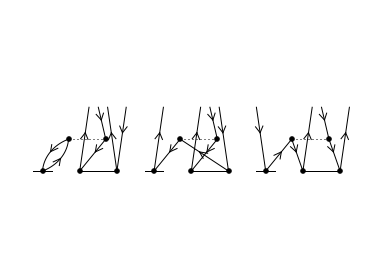
\includegraphics[max size={\textwidth}{\textheight}]{ccalgebra_for_web_files/ccalgebra_for_web_22_0.png}
    \par
    \end{center}
    
            \end{InvisibleVerbatim}
            
        
    


    % Make sure that atleast 4 lines are below the HR
    \needspace{4\baselineskip}

    
        \vspace{6pt}
        \makebox[0.1\linewidth]{\smaller\hfill\tt\color{nbframe-in-prompt}In\hspace{4pt}{[}10{]}:\hspace{4pt}}\\*
        \vspace{-2.65\baselineskip}
        \begin{ColorVerbatim}
            \vspace{-0.7\baselineskip}
            \begin{Verbatim}[commandchars=\\\{\}]
\PY{k}{print} \PY{n}{contraction}\PY{o}{.}\PY{n}{code}\PY{p}{(}\PY{l+m+mi}{0}\PY{p}{)}
\end{Verbatim}

            
                \vspace{-0.2\baselineskip}
            
        \end{ColorVerbatim}
    

    

        % If the first block is an image, minipage the image.  Else
        % request a certain amount of space for the input text.
        \needspace{4\baselineskip}
        
        

            % Add document contents.
            
                \begin{InvisibleVerbatim}
                \vspace{-0.5\baselineskip}
\begin{alltt}
double CCa = 0.0;
for(int d = nElectrons; d < nStates; d ++)\{
    for(int k = 0; k < nElectrons; k ++)\{
        for(int c = nElectrons; c < nStates; c ++)\{
            CCa += v2(a,k)(c,d)*t1(c)(k)*t2(d,b)(i,j)-(v2(b,k)(c,d)*t1
(c)(k)*t2(d,a)(i,j));
        \}
    \}
\}
double CCa *= -1.000000;

\end{alltt}

            \end{InvisibleVerbatim}
            
        
    
\subsubsection{4. Higher level
functions.}\label{higher-level-functions.}

While the examples above deal with single filaments of the hamiltionian,
the full normal ordered hamiltionian will be a sum of more than one such
filaments. When setting up the CC equations we will need to consider the
connection between all this filaments and all terms in the expansion of
the exponential ansatz.

To handle this, we will employ some complementary functions below.\subsubsection{4.1 Complementary functions -
expand\_ansatz()}\label{complementary-functions---expandux5fansatz}

The function expand\_ansatz(list, int) takes as input a list with each
element a list-embraced operator - typically cluster operators in the
cluster expansion. The integer value indicates at what order the
expansion should be truncated. Note that (1) very high values of int
will most likely cause a system overload, and (2) when using a
hamiltonian with at most two-body interactions, no higher orders than 4
is needed due to the fact that the hamiltionian needs to connect to all
cluster-operators to its right.

In the example below it is shown that any list of lists may be used as
input for the expand\_ansatz() function:

    % Make sure that atleast 4 lines are below the HR
    \needspace{4\baselineskip}

    
        \vspace{6pt}
        \makebox[0.1\linewidth]{\smaller\hfill\tt\color{nbframe-in-prompt}In\hspace{4pt}{[}11{]}:\hspace{4pt}}\\*
        \vspace{-2.65\baselineskip}
        \begin{ColorVerbatim}
            \vspace{-0.7\baselineskip}
            \begin{Verbatim}[commandchars=\\\{\}]
\PY{k}{print} \PY{n}{expand\PYZus{}ansatz}\PY{p}{(}\PY{p}{[}\PY{p}{[}\PY{l+s}{\PYZdq{}}\PY{l+s}{a}\PY{l+s}{\PYZdq{}}\PY{p}{]}\PY{p}{,}\PY{p}{[}\PY{l+s}{\PYZdq{}}\PY{l+s}{b}\PY{l+s}{\PYZdq{}}\PY{p}{]}\PY{p}{]}\PY{p}{,} \PY{l+m+mi}{3}\PY{p}{)}
\end{Verbatim}

            
                \vspace{-0.2\baselineskip}
            
        \end{ColorVerbatim}
    

    

        % If the first block is an image, minipage the image.  Else
        % request a certain amount of space for the input text.
        \needspace{4\baselineskip}
        
        

            % Add document contents.
            
                \begin{InvisibleVerbatim}
                \vspace{-0.5\baselineskip}
\begin{alltt}[['a'], ['b'], ['a', 'a'], ['a', 'b'], ['b', 'a'], ['b', 'b'], ['a',
'a', 'a'], ['a', 'a', 'b'], ['a', 'b', 'a'], ['a', 'b', 'b'], ['b',
'a', 'a'], ['b', 'a', 'b'], ['b', 'b', 'a'], ['b', 'b', 'b']]
\end{alltt}

            \end{InvisibleVerbatim}
            
        
    
\subsubsection{4.2 Complementary functions -
normal\_ordered\_hamiltonian()}\label{complementary-functions---normalux5forderedux5fhamiltonian}

This function is called without any arguments and returns a prewritten
list of operators corresponding to the normal ordered hamiltonian in
S-B. (p.280-281). It may be illustrative to see how it is set up while
comparing each element to its diagrammatic counterpart:

    % Make sure that atleast 4 lines are below the HR
    \needspace{4\baselineskip}

    
        \vspace{6pt}
        \makebox[0.1\linewidth]{\smaller\hfill\tt\color{nbframe-in-prompt}In\hspace{4pt}{[}12{]}:\hspace{4pt}}\\*
        \vspace{-2.65\baselineskip}
        \begin{ColorVerbatim}
            \vspace{-0.7\baselineskip}
            \begin{Verbatim}[commandchars=\\\{\}]
\PY{k}{def} \PY{n+nf}{normal\PYZus{}ordered\PYZus{}hamiltonian}\PY{p}{(}\PY{p}{)}\PY{p}{:}
    \PY{c}{\PYZsh{}These elements corresponds to (9.105) in S\PYZhy{}B:}
    \PY{n}{F1} \PY{o}{=} \PY{n}{Operator}\PY{p}{(}\PY{p}{[}\PY{l+m+mi}{1}\PY{p}{]}\PY{p}{,}\PY{p}{[}\PY{l+m+mi}{1}\PY{p}{]}\PY{p}{)}     \PY{c}{\PYZsh{}Excitation level: 0}
    \PY{n}{F2} \PY{o}{=} \PY{n}{Operator}\PY{p}{(}\PY{p}{[}\PY{o}{\PYZhy{}}\PY{l+m+mi}{1}\PY{p}{]}\PY{p}{,}\PY{p}{[}\PY{o}{\PYZhy{}}\PY{l+m+mi}{1}\PY{p}{]}\PY{p}{)}   \PY{c}{\PYZsh{}E:0}
    \PY{n}{F3} \PY{o}{=} \PY{n}{Operator}\PY{p}{(}\PY{p}{[}\PY{p}{]}\PY{p}{,}\PY{p}{[}\PY{l+m+mi}{1}\PY{p}{,}\PY{o}{\PYZhy{}}\PY{l+m+mi}{1}\PY{p}{]}\PY{p}{)}   \PY{c}{\PYZsh{}E:+1}
    \PY{n}{F4} \PY{o}{=} \PY{n}{Operator}\PY{p}{(}\PY{p}{[}\PY{l+m+mi}{1}\PY{p}{,}\PY{o}{\PYZhy{}}\PY{l+m+mi}{1}\PY{p}{]}\PY{p}{,}\PY{p}{[}\PY{p}{]}\PY{p}{)}   \PY{c}{\PYZsh{}E:\PYZhy{}1}
    
    \PY{c}{\PYZsh{}These elements correspond to (9.107) in S\PYZhy{}B:}
    \PY{n}{V1} \PY{o}{=} \PY{n}{Operator}\PY{p}{(}\PY{p}{[}\PY{l+m+mi}{1}\PY{p}{,}\PY{l+m+mi}{1}\PY{p}{]}\PY{p}{,}\PY{p}{[}\PY{l+m+mi}{1}\PY{p}{,}\PY{l+m+mi}{1}\PY{p}{]}\PY{p}{)}     \PY{c}{\PYZsh{}E:0}
    \PY{n}{V2} \PY{o}{=} \PY{n}{Operator}\PY{p}{(}\PY{p}{[}\PY{o}{\PYZhy{}}\PY{l+m+mi}{1}\PY{p}{,}\PY{o}{\PYZhy{}}\PY{l+m+mi}{1}\PY{p}{]}\PY{p}{,}\PY{p}{[}\PY{o}{\PYZhy{}}\PY{l+m+mi}{1}\PY{p}{,}\PY{o}{\PYZhy{}}\PY{l+m+mi}{1}\PY{p}{]}\PY{p}{)} \PY{c}{\PYZsh{}E:0}
    \PY{n}{V3} \PY{o}{=} \PY{n}{Operator}\PY{p}{(}\PY{p}{[}\PY{l+m+mi}{1}\PY{p}{,}\PY{o}{\PYZhy{}}\PY{l+m+mi}{1}\PY{p}{]}\PY{p}{,}\PY{p}{[}\PY{l+m+mi}{1}\PY{p}{,}\PY{o}{\PYZhy{}}\PY{l+m+mi}{1}\PY{p}{]}\PY{p}{)}   \PY{c}{\PYZsh{}E:0}
    
    \PY{n}{V4} \PY{o}{=} \PY{n}{Operator}\PY{p}{(}\PY{p}{[}\PY{l+m+mi}{1}\PY{p}{]}\PY{p}{,}\PY{p}{[}\PY{l+m+mi}{1}\PY{p}{,}\PY{l+m+mi}{1}\PY{p}{,}\PY{o}{\PYZhy{}}\PY{l+m+mi}{1}\PY{p}{]}\PY{p}{)}    \PY{c}{\PYZsh{}E:+1}
    \PY{n}{V5} \PY{o}{=} \PY{n}{Operator}\PY{p}{(}\PY{p}{[}\PY{l+m+mi}{1}\PY{p}{,}\PY{l+m+mi}{1}\PY{p}{,}\PY{o}{\PYZhy{}}\PY{l+m+mi}{1}\PY{p}{]}\PY{p}{,}\PY{p}{[}\PY{l+m+mi}{1}\PY{p}{]}\PY{p}{)}    \PY{c}{\PYZsh{}E:\PYZhy{}1}
    \PY{n}{V7} \PY{o}{=} \PY{n}{Operator}\PY{p}{(}\PY{p}{[}\PY{l+m+mi}{1}\PY{p}{,}\PY{o}{\PYZhy{}}\PY{l+m+mi}{1}\PY{p}{,}\PY{o}{\PYZhy{}}\PY{l+m+mi}{1}\PY{p}{]}\PY{p}{,}\PY{p}{[}\PY{o}{\PYZhy{}}\PY{l+m+mi}{1}\PY{p}{]}\PY{p}{)}  \PY{c}{\PYZsh{}E:\PYZhy{}1}
    \PY{n}{V6} \PY{o}{=} \PY{n}{Operator}\PY{p}{(}\PY{p}{[}\PY{o}{\PYZhy{}}\PY{l+m+mi}{1}\PY{p}{]}\PY{p}{,}\PY{p}{[}\PY{l+m+mi}{1}\PY{p}{,}\PY{o}{\PYZhy{}}\PY{l+m+mi}{1}\PY{p}{,}\PY{o}{\PYZhy{}}\PY{l+m+mi}{1}\PY{p}{]}\PY{p}{)}  \PY{c}{\PYZsh{}E:+1}
    
    \PY{n}{V9} \PY{o}{=} \PY{n}{Operator}\PY{p}{(}\PY{p}{[}\PY{l+m+mi}{1}\PY{p}{,}\PY{l+m+mi}{1}\PY{p}{,}\PY{o}{\PYZhy{}}\PY{l+m+mi}{1}\PY{p}{,}\PY{o}{\PYZhy{}}\PY{l+m+mi}{1}\PY{p}{]}\PY{p}{,}\PY{p}{[}\PY{p}{]}\PY{p}{)}  \PY{c}{\PYZsh{}E:\PYZhy{}2}
    \PY{n}{V8} \PY{o}{=} \PY{n}{Operator}\PY{p}{(}\PY{p}{[}\PY{p}{]}\PY{p}{,}\PY{p}{[}\PY{l+m+mi}{1}\PY{p}{,}\PY{l+m+mi}{1}\PY{p}{,}\PY{o}{\PYZhy{}}\PY{l+m+mi}{1}\PY{p}{,}\PY{o}{\PYZhy{}}\PY{l+m+mi}{1}\PY{p}{]}\PY{p}{)}  \PY{c}{\PYZsh{}E:+2}
    
    \PY{k}{return} \PY{p}{[}\PY{n}{F1}\PY{p}{,}\PY{n}{F2}\PY{p}{,}\PY{n}{F3}\PY{p}{,}\PY{n}{F4}\PY{p}{,}\PY{n}{V1}\PY{p}{,}\PY{n}{V2}\PY{p}{,}\PY{n}{V3}\PY{p}{,}\PY{n}{V4}\PY{p}{,}\PY{n}{V5}\PY{p}{,}\PY{n}{V6}\PY{p}{,}\PY{n}{V7}\PY{p}{,}\PY{n}{V8}\PY{p}{,}\PY{n}{V9}\PY{p}{]}   
\end{Verbatim}

            
                \vspace{-0.2\baselineskip}
            
        \end{ColorVerbatim}
    
\subsubsection{4.3 Complementary functions -
cluster\_operator()}\label{complementary-functions---clusterux5foperator}

To quickly set up the \(T = T_1 + T_2 + ...\) cluster operator, one may
call the cluster\_operator() function. This function will return a list
of cluster operators, each in the order specified in the function
arguments. Some examples are given below:

    % Make sure that atleast 4 lines are below the HR
    \needspace{4\baselineskip}

    
        \vspace{6pt}
        \makebox[0.1\linewidth]{\smaller\hfill\tt\color{nbframe-in-prompt}In\hspace{4pt}{[}13{]}:\hspace{4pt}}\\*
        \vspace{-2.65\baselineskip}
        \begin{ColorVerbatim}
            \vspace{-0.7\baselineskip}
            \begin{Verbatim}[commandchars=\\\{\}]
\PY{k}{print} \PY{n}{cluster\PYZus{}operator}\PY{p}{(}\PY{p}{[}\PY{l+m+mi}{1}\PY{p}{,}\PY{l+m+mi}{2}\PY{p}{,}\PY{l+m+mi}{3}\PY{p}{]}\PY{p}{)} \PY{c}{\PYZsh{} returns [T\PYZus{}1, T\PYZus{}2, T\PYZus{}3]}
\end{Verbatim}

            
                \vspace{-0.2\baselineskip}
            
        \end{ColorVerbatim}
    

    

        % If the first block is an image, minipage the image.  Else
        % request a certain amount of space for the input text.
        \needspace{4\baselineskip}
        
        

            % Add document contents.
            
                \begin{InvisibleVerbatim}
                \vspace{-0.5\baselineskip}
\begin{alltt}[[<\_\_main\_\_.Operator instance at 0x000000000506F248>],
[<\_\_main\_\_.Operator instance at 0x000000000506F708>],
[<\_\_main\_\_.Operator instance at 0x000000000506F888>]]
\end{alltt}

            \end{InvisibleVerbatim}
            
        
    
\subsubsection{5. Functions for deriving the CC
equations.}\label{functions-for-deriving-the-cc-equations.}

So far we have introduced all the functionality needed to set up the
elements in the equations, but we have not set up the equations
themselves. To do this, we need yet another pair of functions.

When deriving the equations we need to consider all possible connections
between hamiltonian filaments and combinations of cluster operators in
the cluster expansion. Currently there are two such higher level
functions available.\subsubsection{5.1 The combine\_all()
function}\label{the-combineux5fall-function}

Combining all elements in the normal ordered hamiltonian with all
elements in the cluster expansion will produce a high number of excited
slater determinants. To see all of these we may use the combine\_all()
function. In the following example we set up a normal ordered
hamiltonian and a list of list of cluster operators, and then we find
all combinations between these operators, representing them
mathematically.

    % Make sure that atleast 4 lines are below the HR
    \needspace{4\baselineskip}

    
        \vspace{6pt}
        \makebox[0.1\linewidth]{\smaller\hfill\tt\color{nbframe-in-prompt}In\hspace{4pt}{[}14{]}:\hspace{4pt}}\\*
        \vspace{-2.65\baselineskip}
        \begin{ColorVerbatim}
            \vspace{-0.7\baselineskip}
            \begin{Verbatim}[commandchars=\\\{\}]
\PY{n}{H} \PY{o}{=} \PY{n}{normal\PYZus{}ordered\PYZus{}hamiltonian}\PY{p}{(}\PY{p}{)}
\PY{n}{T\PYZus{}1} \PY{o}{=} \PY{n}{Operator}\PY{p}{(}\PY{p}{[}\PY{p}{]}\PY{p}{,}\PY{p}{[}\PY{l+m+mi}{1}\PY{p}{,}\PY{o}{\PYZhy{}}\PY{l+m+mi}{1}\PY{p}{]}\PY{p}{)}      \PY{c}{\PYZsh{}The T\PYZus{}1 cluster operator}
\PY{n}{T\PYZus{}2} \PY{o}{=} \PY{n}{Operator}\PY{p}{(}\PY{p}{[}\PY{p}{]}\PY{p}{,}\PY{p}{[}\PY{l+m+mi}{1}\PY{p}{,}\PY{l+m+mi}{1}\PY{p}{,}\PY{o}{\PYZhy{}}\PY{l+m+mi}{1}\PY{p}{,}\PY{o}{\PYZhy{}}\PY{l+m+mi}{1}\PY{p}{]}\PY{p}{)} \PY{c}{\PYZsh{}The T\PYZus{}2 operator; all lists must be normal ordered}
\PY{n}{expT} \PY{o}{=} \PY{n}{expand\PYZus{}ansatz}\PY{p}{(}\PY{p}{[}\PY{p}{[}\PY{n}{T\PYZus{}1}\PY{p}{]}\PY{p}{,}\PY{p}{[}\PY{n}{T\PYZus{}2}\PY{p}{]}\PY{p}{]}\PY{p}{,} \PY{l+m+mi}{1}\PY{p}{)}
\PY{n}{tx} \PY{o}{=} \PY{n}{combine\PYZus{}all}\PY{p}{(}\PY{n}{H}\PY{p}{,}\PY{n}{expT}\PY{p}{,} \PY{p}{[}\PY{l+m+mi}{1}\PY{p}{,}\PY{l+m+mi}{0}\PY{p}{,}\PY{l+m+mi}{0}\PY{p}{,}\PY{l+m+mi}{0}\PY{p}{]}\PY{p}{)} \PY{c}{\PYZsh{}The list is explained below}
\PY{n}{S} \PY{o}{=} \PY{l+s}{\PYZdq{}}\PY{l+s}{0 = }\PY{l+s}{\PYZdq{}}
\PY{k}{for} \PY{n}{i} \PY{o+ow}{in} \PY{n}{tx}\PY{p}{:}
    \PY{n}{S}\PY{o}{+}\PY{o}{=} \PY{n}{i}
\PY{n}{Math}\PY{p}{(}\PY{n}{S}\PY{p}{)}
\end{Verbatim}

            
                \vspace{-0.2\baselineskip}
            
        \end{ColorVerbatim}
    

    

        % If the first block is an image, minipage the image.  Else
        % request a certain amount of space for the input text.
        \needspace{4\baselineskip}
        
        

            % Add document contents.
            
                \makebox[0.1\linewidth]{\smaller\hfill\tt\color{nbframe-out-prompt}Out\hspace{4pt}{[}14{]}:\hspace{4pt}}\\*
                \vspace{-2.55\baselineskip}\begin{InvisibleVerbatim}
                \vspace{-0.5\baselineskip}
$$0 = \frac{1}{1} \sum_{c} \langle a || c \rangle t_{i}^{c}P(ba)\frac{-1}{1} \sum_{c} \langle a || c \rangle t_{ij}^{cb}\frac{-1}{1} \sum_{k} \langle k || i \rangle t_{k}^{a}P(ij)\frac{1}{1} \sum_{k} \langle k || j \rangle t_{ik}^{ab}\frac{1}{1} \sum_{ck} \langle k || c \rangle t_{k}^{c}\frac{1}{1} \sum_{ck} \langle k || c \rangle t_{ik}^{ca}\frac{1}{2} \sum_{cd} \langle ab || cd \rangle t_{ij}^{cd}\frac{1}{2} \sum_{kl} \langle kl || ij \rangle t_{kl}^{ab}\frac{-1}{1} \sum_{ck} \langle ak || ci \rangle t_{k}^{c}P(ba)P(ij)\frac{-1}{1} \sum_{ck} \langle ak || cj \rangle t_{ik}^{cb}P(ij)\frac{1}{1} \sum_{c} \langle a || c \rangle t_{i}^{c}P(ba)P(bz)P(iw)P(jw)\frac{-1}{1} \sum_{c} \langle a || c \rangle t_{ij}^{cb}\frac{1}{2} \sum_{cdk} \langle ak || cd \rangle t_{ik}^{cd}P(ab)\frac{-1}{1} \sum_{k} \langle k || i \rangle t_{k}^{a}P(az)P(bz)P(ij)P(iw)\frac{1}{1} \sum_{k} \langle k || j \rangle t_{ik}^{ab}\frac{-1}{2} \sum_{ckl} \langle kl || ci \rangle t_{kl}^{ca}\frac{1}{4} \sum_{cdkl} \langle kl || cd \rangle t_{kl}^{cd}$$
            \end{InvisibleVerbatim}
            
        
    
The combine\_all() function is called with the two listst of operators
as parameters and a maybe cryptic list with instructions on how to
represent the combinations. The list of instructions works as follows:

{[}0,0,0,0{]} - Produce no representations, only iterate through all
connections

{[}1,0,0,0{]} - Return a string of latex-formatted expression for each
connection.

{[}0,1,0,0{]} - Plot all diagrams in same figure.

{[}0,2,0,0{]} - Plot each diagram in a separate figure. (May produce a
lot of diagrams.)

{[}0,0,1,0{]} - Display the report for each diagram. (Explained in
section 3 above)

{[}0,0,0,1{]} - Print out the code for all diagrams.

The arguments may of course be combined if more than one index is set to
non-zero values:

{[}1,2,1,1{]} - Return string, plot separate diagrams, show report and
print code.

\textbf{Important:} This function is not very practical, and will most
likely cause a memory overload if applied to diagrams with many
permutations in the sums (due to the length of the C++ string.). For all
practical purposes, the combine\_to\_excitation() function should be
utilized in its place.\subsubsection{5.2 The combine\_to\_excitation()
function}\label{the-combineux5ftoux5fexcitation-function}

While the combine\_all() function might have som educational value, it
will show a lot more diagrams than what we in reality seek. When setting
up the energy- and amplitide equations, we seek only contributions that
correspond to certain excitation levels. This is beause the application
of the exponential ansatz connected to the hamiltonian will produce a
variety of excited states using the virtual orbitals in the SD, and when
solving for the amplitudes we need to project these states down on a bra
SD of the target excited state. (please forgive my messy formulation)

To find only the excitation levels of interest, i.e.~the contributions
to each equation, we may write (using the same functions as above):

    % Make sure that atleast 4 lines are below the HR
    \needspace{4\baselineskip}

    
        \vspace{6pt}
        \makebox[0.1\linewidth]{\smaller\hfill\tt\color{nbframe-in-prompt}In\hspace{4pt}{[}15{]}:\hspace{4pt}}\\*
        \vspace{-2.65\baselineskip}
        \begin{ColorVerbatim}
            \vspace{-0.7\baselineskip}
            \begin{Verbatim}[commandchars=\\\{\}]
\PY{n}{tx} \PY{o}{=} \PY{n}{combine\PYZus{}to\PYZus{}excitation}\PY{p}{(}\PY{n}{H}\PY{p}{,}\PY{n}{expT}\PY{p}{,}\PY{l+m+mi}{1}\PY{p}{,} \PY{p}{[}\PY{l+m+mi}{1}\PY{p}{,}\PY{l+m+mi}{0}\PY{p}{,}\PY{l+m+mi}{0}\PY{p}{,}\PY{l+m+mi}{0}\PY{p}{]}\PY{p}{)} \PY{c}{\PYZsh{}All combinations that produce excitation level 1}
\PY{n}{S} \PY{o}{=} \PY{l+s}{\PYZdq{}}\PY{l+s}{0 =}\PY{l+s}{\PYZdq{}}
\PY{k}{for} \PY{n}{i} \PY{o+ow}{in} \PY{n}{tx}\PY{p}{:}
    \PY{n}{S}\PY{o}{+}\PY{o}{=} \PY{l+s}{\PYZdq{}}\PY{l+s}{+}\PY{l+s}{\PYZdq{}}\PY{o}{+} \PY{n}{i}
\PY{n}{Math}\PY{p}{(}\PY{n}{S}\PY{p}{)}
\end{Verbatim}

            
                \vspace{-0.2\baselineskip}
            
        \end{ColorVerbatim}
    

    

        % If the first block is an image, minipage the image.  Else
        % request a certain amount of space for the input text.
        \needspace{4\baselineskip}
        
        

            % Add document contents.
            
                \makebox[0.1\linewidth]{\smaller\hfill\tt\color{nbframe-out-prompt}Out\hspace{4pt}{[}15{]}:\hspace{4pt}}\\*
                \vspace{-2.55\baselineskip}\begin{InvisibleVerbatim}
                \vspace{-0.5\baselineskip}
$$0 =+\frac{1}{1} \sum_{c} \langle a || c \rangle t_{i}^{c}+\frac{-1}{1} \sum_{k} \langle k || i \rangle t_{k}^{a}+\frac{1}{1} \sum_{ck} \langle k || c \rangle t_{ik}^{ca}+\frac{-1}{1} \sum_{ck} \langle ak || ci \rangle t_{k}^{c}+\frac{1}{2} \sum_{cdk} \langle ak || cd \rangle t_{ik}^{cd}+\frac{-1}{2} \sum_{ckl} \langle kl || ci \rangle t_{kl}^{ca}$$
            \end{InvisibleVerbatim}
            
        
    
And voila! This is basically the T1 amplitude equation in the CCSD
truncation.

Note the third argument, setting the excitation level of interest to 1.
All the sums above have this excitation level. We may also display these
6 contributions to the \(t_1\) amplitude equation as diagrams:

    % Make sure that atleast 4 lines are below the HR
    \needspace{4\baselineskip}

    
        \vspace{6pt}
        \makebox[0.1\linewidth]{\smaller\hfill\tt\color{nbframe-in-prompt}In\hspace{4pt}{[}16{]}:\hspace{4pt}}\\*
        \vspace{-2.65\baselineskip}
        \begin{ColorVerbatim}
            \vspace{-0.7\baselineskip}
            \begin{Verbatim}[commandchars=\\\{\}]
\PY{n}{tx} \PY{o}{=} \PY{n}{combine\PYZus{}to\PYZus{}excitation}\PY{p}{(}\PY{n}{H}\PY{p}{,}\PY{n}{expT}\PY{p}{,}\PY{l+m+mi}{1}\PY{p}{,} \PY{p}{[}\PY{l+m+mi}{0}\PY{p}{,}\PY{l+m+mi}{1}\PY{p}{,}\PY{l+m+mi}{0}\PY{p}{,}\PY{l+m+mi}{0}\PY{p}{]}\PY{p}{)} \PY{c}{\PYZsh{}All combinations that produce excitation level 1}
\end{Verbatim}

            
                \vspace{-0.2\baselineskip}
            
        \end{ColorVerbatim}
    

    

        % If the first block is an image, minipage the image.  Else
        % request a certain amount of space for the input text.
        \needspace{4\baselineskip}
        
        

            % Add document contents.
            
                \begin{InvisibleVerbatim}
                \vspace{-0.5\baselineskip}
    \begin{center}
    
\includegraphics[max size={\textwidth}{\textheight}]{ccalgebra_for_web_files/ccalgebra_for_web_38_0.png}
    \par
    \end{center}
    
            \end{InvisibleVerbatim}
            
                \begin{InvisibleVerbatim}
                \vspace{-0.5\baselineskip}
    \begin{center}
    
\includegraphics[max size={\textwidth}{\textheight}]{ccalgebra_for_web_files/ccalgebra_for_web_38_1.png}
    \par
    \end{center}
    
            \end{InvisibleVerbatim}
            
                \begin{InvisibleVerbatim}
                \vspace{-0.5\baselineskip}
    \begin{center}
    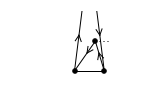
\includegraphics[max size={\textwidth}{\textheight}]{ccalgebra_for_web_files/ccalgebra_for_web_38_2.png}
    \par
    \end{center}
    
            \end{InvisibleVerbatim}
            
                \begin{InvisibleVerbatim}
                \vspace{-0.5\baselineskip}
    \begin{center}
    
\includegraphics[max size={\textwidth}{\textheight}]{ccalgebra_for_web_files/ccalgebra_for_web_38_3.png}
    \par
    \end{center}
    
            \end{InvisibleVerbatim}
            
                \begin{InvisibleVerbatim}
                \vspace{-0.5\baselineskip}
    \begin{center}
    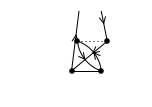
\includegraphics[max size={\textwidth}{\textheight}]{ccalgebra_for_web_files/ccalgebra_for_web_38_4.png}
    \par
    \end{center}
    
            \end{InvisibleVerbatim}
            
                \begin{InvisibleVerbatim}
                \vspace{-0.5\baselineskip}
    \begin{center}
    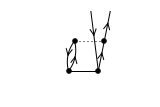
\includegraphics[max size={\textwidth}{\textheight}]{ccalgebra_for_web_files/ccalgebra_for_web_38_5.png}
    \par
    \end{center}
    
            \end{InvisibleVerbatim}
            
        
    
\subsubsection{6. Deriving the CCD
equations}\label{deriving-the-ccd-equations}

We are now ready to derive the full CCD equations. We perform the
operations in two separate cells, one for the energy and another for the
\(t_2\) amplitude equation. This example might be considered typical for
a session where we want to produce some code for a C++ implementation
for CCD.

    % Make sure that atleast 4 lines are below the HR
    \needspace{4\baselineskip}

    
        \vspace{6pt}
        \makebox[0.1\linewidth]{\smaller\hfill\tt\color{nbframe-in-prompt}In\hspace{4pt}{[}46{]}:\hspace{4pt}}\\*
        \vspace{-2.65\baselineskip}
        \begin{ColorVerbatim}
            \vspace{-0.7\baselineskip}
            \begin{Verbatim}[commandchars=\\\{\}]
\PY{n}{H} \PY{o}{=} \PY{n}{normal\PYZus{}ordered\PYZus{}hamiltonian}\PY{p}{(}\PY{p}{)}
\PY{n}{T\PYZus{}2} \PY{o}{=} \PY{n}{Operator}\PY{p}{(}\PY{p}{[}\PY{p}{]}\PY{p}{,}\PY{p}{[}\PY{l+m+mi}{1}\PY{p}{,}\PY{l+m+mi}{1}\PY{p}{,}\PY{o}{\PYZhy{}}\PY{l+m+mi}{1}\PY{p}{,}\PY{o}{\PYZhy{}}\PY{l+m+mi}{1}\PY{p}{]}\PY{p}{)} 
\PY{n}{expT} \PY{o}{=} \PY{n}{expand\PYZus{}ansatz}\PY{p}{(}\PY{p}{[}\PY{p}{[}\PY{n}{T\PYZus{}2}\PY{p}{]}\PY{p}{]}\PY{p}{,} \PY{l+m+mi}{4}\PY{p}{)} \PY{c}{\PYZsh{}Natural truncation}
\PY{n}{tx} \PY{o}{=} \PY{n}{combine\PYZus{}to\PYZus{}excitation}\PY{p}{(}\PY{n}{H}\PY{p}{,}\PY{n}{expT}\PY{p}{,} \PY{l+m+mi}{0}\PY{p}{,} \PY{p}{[}\PY{l+m+mi}{1}\PY{p}{,}\PY{l+m+mi}{1}\PY{p}{,}\PY{l+m+mi}{0}\PY{p}{,}\PY{l+m+mi}{0}\PY{p}{]}\PY{p}{)} \PY{c}{\PYZsh{}The list is explained below}
\PY{n}{S} \PY{o}{=} \PY{l+s}{\PYZdq{}}\PY{l+s}{0 = }\PY{l+s}{\PYZdq{}}
\PY{k}{for} \PY{n}{i} \PY{o+ow}{in} \PY{n}{tx}\PY{p}{:}
    \PY{n}{S}\PY{o}{+}\PY{o}{=} \PY{l+s}{\PYZdq{}}\PY{l+s}{+}\PY{l+s}{\PYZdq{}} \PY{o}{+} \PY{n}{i}
\PY{n}{Math}\PY{p}{(}\PY{n}{S}\PY{p}{)}
\end{Verbatim}

            
                \vspace{-0.2\baselineskip}
            
        \end{ColorVerbatim}
    

    

        % If the first block is an image, minipage the image.  Else
        % request a certain amount of space for the input text.
        \needspace{4\baselineskip}
        
        

            % Add document contents.
            
                \begin{InvisibleVerbatim}
                \vspace{-0.5\baselineskip}
    \begin{center}
    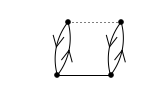
\includegraphics[max size={\textwidth}{\textheight}]{ccalgebra_for_web_files/ccalgebra_for_web_40_0.png}
    \par
    \end{center}
    
            \end{InvisibleVerbatim}
            
                \makebox[0.1\linewidth]{\smaller\hfill\tt\color{nbframe-out-prompt}Out\hspace{4pt}{[}46{]}:\hspace{4pt}}\\*
                \vspace{-2.55\baselineskip}\begin{InvisibleVerbatim}
                \vspace{-0.5\baselineskip}
$$0 = +\frac{1}{4} \sum_{cdkl} \langle kl || cd \rangle t_{kl}^{cd}$$
            \end{InvisibleVerbatim}
            
        
    
As expected, we find only one contribution to the energy expression.
People familiar with diagrammatic notation quickly recognize the CCD
energy above. Now for the \(t_2\) amplitude equation (in the example we
return the code):

    % Make sure that atleast 4 lines are below the HR
    \needspace{4\baselineskip}

    
        \vspace{6pt}
        \makebox[0.1\linewidth]{\smaller\hfill\tt\color{nbframe-in-prompt}In\hspace{4pt}{[}47{]}:\hspace{4pt}}\\*
        \vspace{-2.65\baselineskip}
        \begin{ColorVerbatim}
            \vspace{-0.7\baselineskip}
            \begin{Verbatim}[commandchars=\\\{\}]
\PY{c}{\PYZsh{}tx = combine\PYZus{}to\PYZus{}excitation(H,expT, 2, [0,0,0,1]) \PYZsh{}The list is explained below}
\PY{n}{tx} \PY{o}{=} \PY{n}{combine\PYZus{}to\PYZus{}excitation}\PY{p}{(}\PY{n}{H}\PY{p}{,}\PY{n}{expT}\PY{p}{,} \PY{l+m+mi}{2}\PY{p}{,} \PY{p}{[}\PY{l+m+mi}{1}\PY{p}{,}\PY{l+m+mi}{0}\PY{p}{,}\PY{l+m+mi}{0}\PY{p}{,}\PY{l+m+mi}{1}\PY{p}{]}\PY{p}{)} \PY{c}{\PYZsh{}The list is explained below}
\PY{n}{S} \PY{o}{=} \PY{l+s}{\PYZdq{}}\PY{l+s}{0 = }\PY{l+s}{\PYZdq{}}
\PY{k}{for} \PY{n}{i} \PY{o+ow}{in} \PY{n}{tx}\PY{p}{:}
    \PY{n}{S}\PY{o}{+}\PY{o}{=} \PY{l+s}{\PYZdq{}}\PY{l+s}{+}\PY{l+s}{\PYZdq{}} \PY{o}{+} \PY{n}{i}
\PY{n}{Math}\PY{p}{(}\PY{n}{S}\PY{p}{)}
\end{Verbatim}

            
                \vspace{-0.2\baselineskip}
            
        \end{ColorVerbatim}
    

    

        % If the first block is an image, minipage the image.  Else
        % request a certain amount of space for the input text.
        \needspace{4\baselineskip}
        
        

            % Add document contents.
            
                \begin{InvisibleVerbatim}
                \vspace{-0.5\baselineskip}
\begin{alltt}
double CC0\_0a = 0.0;
for(int c = nElectrons; c < nStates; c ++)\{
    CC0\_0a += vmin1(a)(c)*tf2(c,b)(i,j)-(vmin1(b)(c)*tf2(c,a)(i,j));
\}
CC0\_0a *= -1.000000;


double CC1\_0a = 0.0;
for(int k = 0; k < nElectrons; k ++)\{
    CC1\_0a += vmin1(k)(j)*tf2(a,b)(i,k)-(vmjn1(k)(i)*tf2(a,b)(j,k));
\}
CC1\_0a *= 1.000000;


double CC4\_0a = 0.0;
for(int d = nElectrons; d < nStates; d ++)\{
    for(int c = nElectrons; c < nStates; c ++)\{
        CC4\_0a += vmin2(a,b)(c,d)*tf2(c,d)(i,j);
    \}
\}
CC4\_0a *= 0.500000;


double CC5\_0a = 0.0;
for(int l = 0; l < nElectrons; l ++)\{
    for(int k = 0; k < nElectrons; k ++)\{
        CC5\_0a += vmin2(k,l)(i,j)*tf2(a,b)(k,l);
    \}
\}
CC5\_0a *= 0.500000;


double CC6\_0a = 0.0;
for(int k = 0; k < nElectrons; k ++)\{
    for(int c = nElectrons; c < nStates; c ++)\{
        CC6\_0a += vmin2(a,k)(c,j)*tf2(c,b)(i,k)-(vmin2(b,k)(c,j)*tf2(c
,a)(i,k))-(vmjn2(a,k)(c,i)*tf2(c,b)(j,k)-(vmjn2(b,k)(c,i)*tf2(c,a)(j,k
)));
    \}
\}
CC6\_0a *= -1.000000;


double CC12\_1a = 0.0;
for(int l = 0; l < nElectrons; l ++)\{
    for(int k = 0; k < nElectrons; k ++)\{
        for(int d = nElectrons; d < nStates; d ++)\{
            for(int c = nElectrons; c < nStates; c ++)\{
                CC12\_1a += vmin2(k,l)(c,d)*tf2(c,d)(i,k)*tf2(a,b)(j,l)
-(vmjn2(k,l)(c,d)*tf2(c,d)(j,k)*tf2(a,b)(i,l));
            \}
        \}
    \}
\}
CC12\_1a *= -0.500000;


double CC12\_1b = 0.0;
for(int l = 0; l < nElectrons; l ++)\{
    for(int k = 0; k < nElectrons; k ++)\{
        for(int d = nElectrons; d < nStates; d ++)\{
            for(int c = nElectrons; c < nStates; c ++)\{
                CC12\_1b +=
vmin2(k,l)(c,d)*tf2(c,d)(i,j)*tf2(a,b)(k,l);
            \}
        \}
    \}
\}
CC12\_1b *= 0.250000;


double CC12\_1c = 0.0;
for(int d = nElectrons; d < nStates; d ++)\{
    for(int l = 0; l < nElectrons; l ++)\{
        for(int k = 0; k < nElectrons; k ++)\{
            for(int c = nElectrons; c < nStates; c ++)\{
                CC12\_1c += vmin2(k,l)(c,d)*tf2(c,a)(k,l)*tf2(d,b)(i,j)
-(vmin2(k,l)(c,d)*tf2(c,b)(k,l)*tf2(d,a)(i,j));
            \}
        \}
    \}
\}
CC12\_1c *= -0.500000;


double CC12\_1d = 0.0;
for(int l = 0; l < nElectrons; l ++)\{
    for(int d = nElectrons; d < nStates; d ++)\{
        for(int k = 0; k < nElectrons; k ++)\{
            for(int c = nElectrons; c < nStates; c ++)\{
                CC12\_1d += vmin2(k,l)(c,d)*tf2(c,a)(i,k)*tf2(d,b)(j,l)
-(vmin2(k,l)(c,d)*tf2(c,b)(i,k)*tf2(d,a)(j,l))-(vmjn2(k,l)(c,d)*tf2(c,
a)(j,k)*tf2(d,b)(i,l)-(vmjn2(k,l)(c,d)*tf2(c,b)(j,k)*tf2(d,a)(i,l)));
            \}
        \}
    \}
\}
CC12\_1d *= 0.500000;

\end{alltt}

            \end{InvisibleVerbatim}
            
                \makebox[0.1\linewidth]{\smaller\hfill\tt\color{nbframe-out-prompt}Out\hspace{4pt}{[}47{]}:\hspace{4pt}}\\*
                \vspace{-2.55\baselineskip}\begin{InvisibleVerbatim}
                \vspace{-0.5\baselineskip}
$$0 = +P(ba)\frac{-1}{1} \sum_{c} \langle a || c \rangle t_{ij}^{cb}+P(ij)\frac{1}{1} \sum_{k} \langle k || j \rangle t_{ik}^{ab}+\frac{1}{2} \sum_{cd} \langle ab || cd \rangle t_{ij}^{cd}+\frac{1}{2} \sum_{kl} \langle kl || ij \rangle t_{kl}^{ab}+P(ba)P(ij)\frac{-1}{1} \sum_{ck} \langle ak || cj \rangle t_{ik}^{cb}+P(ij)\frac{-1}{2} \sum_{cdkl} \langle kl || cd \rangle t_{ik}^{cd} t_{jl}^{ab}+\frac{1}{4} \sum_{cdkl} \langle kl || cd \rangle t_{ij}^{cd} t_{kl}^{ab}+P(ab)\frac{-1}{2} \sum_{ckld} \langle kl || cd \rangle t_{kl}^{ca} t_{ij}^{db}+P(ab)P(ij)\frac{1}{2} \sum_{ckdl} \langle kl || cd \rangle t_{ik}^{ca} t_{jl}^{db}$$
            \end{InvisibleVerbatim}
            
        
    
In summary, we see that CCAlgebra has a potential to simplify both the
understanding and implementation of CC-equations. The code above may be
copy-pasted into a C++ class file.

\emph{Update (2.november 2014): The code above was successfully
implemented into my quantum many-body solver
\href{http://www.github.com/audunsh/fys4411}{Fermion Mingle} in C++ with
some minor editing, and the code produced the exact same results I have
obtained from previous benchmarking. This is a proof-of-concept, showing
that CCAlg may be used to write code for solver functions.}\subsubsection{7. Deriving the CCSD
equations}\label{deriving-the-ccsd-equations}

The CCD is considered to be the simplest of the CC equations. When we
also include single excitations, we may derive the CCSD equations. As
the correlation energy is given by completely closed diagrams, we should
only find three possible such connections of operators. This is
confirmed in the example below:

    % Make sure that atleast 4 lines are below the HR
    \needspace{4\baselineskip}

    
        \vspace{6pt}
        \makebox[0.1\linewidth]{\smaller\hfill\tt\color{nbframe-in-prompt}In\hspace{4pt}{[}19{]}:\hspace{4pt}}\\*
        \vspace{-2.65\baselineskip}
        \begin{ColorVerbatim}
            \vspace{-0.7\baselineskip}
            \begin{Verbatim}[commandchars=\\\{\}]
\PY{n}{H} \PY{o}{=} \PY{n}{normal\PYZus{}ordered\PYZus{}hamiltonian}\PY{p}{(}\PY{p}{)} \PY{c}{\PYZsh{}Including one\PYZhy{} and two\PYZhy{}particle interactions}
\PY{n}{expT} \PY{o}{=} \PY{n}{expand\PYZus{}ansatz}\PY{p}{(}\PY{p}{[}\PY{p}{[}\PY{n}{T\PYZus{}1}\PY{p}{]}\PY{p}{,}\PY{p}{[}\PY{n}{T\PYZus{}2}\PY{p}{]}\PY{p}{]}\PY{p}{,}\PY{l+m+mi}{3}\PY{p}{)}  \PY{c}{\PYZsh{}Taylor expand a list of lists to the 3rd order}
\PY{n}{tx} \PY{o}{=} \PY{n}{combine\PYZus{}to\PYZus{}excitation}\PY{p}{(}\PY{n}{H}\PY{p}{,}\PY{n}{expT}\PY{p}{,}\PY{l+m+mi}{0}\PY{p}{,} \PY{p}{[}\PY{l+m+mi}{1}\PY{p}{,}\PY{l+m+mi}{1}\PY{p}{,}\PY{l+m+mi}{0}\PY{p}{,}\PY{l+m+mi}{0}\PY{p}{]}\PY{p}{)} 
\PY{n}{S} \PY{o}{=} \PY{l+s}{\PYZdq{}}\PY{l+s}{0 = }\PY{l+s}{\PYZdq{}}
\PY{k}{for} \PY{n}{i} \PY{o+ow}{in} \PY{n}{tx}\PY{p}{:}
    \PY{n}{S} \PY{o}{+}\PY{o}{=} \PY{l+s}{\PYZdq{}}\PY{l+s}{+}\PY{l+s}{\PYZdq{}} \PY{o}{+} \PY{n}{i}
\PY{n}{Math}\PY{p}{(}\PY{n}{S}\PY{p}{)}
\end{Verbatim}

            
                \vspace{-0.2\baselineskip}
            
        \end{ColorVerbatim}
    

    

        % If the first block is an image, minipage the image.  Else
        % request a certain amount of space for the input text.
        \needspace{4\baselineskip}
        
        

            % Add document contents.
            
                \begin{InvisibleVerbatim}
                \vspace{-0.5\baselineskip}
    \begin{center}
    
\includegraphics[max size={\textwidth}{\textheight}]{ccalgebra_for_web_files/ccalgebra_for_web_45_0.png}
    \par
    \end{center}
    
            \end{InvisibleVerbatim}
            
                \begin{InvisibleVerbatim}
                \vspace{-0.5\baselineskip}
    \begin{center}
    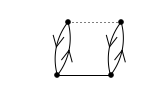
\includegraphics[max size={\textwidth}{\textheight}]{ccalgebra_for_web_files/ccalgebra_for_web_45_1.png}
    \par
    \end{center}
    
            \end{InvisibleVerbatim}
            
                \begin{InvisibleVerbatim}
                \vspace{-0.5\baselineskip}
    \begin{center}
    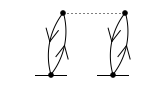
\includegraphics[max size={\textwidth}{\textheight}]{ccalgebra_for_web_files/ccalgebra_for_web_45_2.png}
    \par
    \end{center}
    
            \end{InvisibleVerbatim}
            
                \makebox[0.1\linewidth]{\smaller\hfill\tt\color{nbframe-out-prompt}Out\hspace{4pt}{[}19{]}:\hspace{4pt}}\\*
                \vspace{-2.55\baselineskip}\begin{InvisibleVerbatim}
                \vspace{-0.5\baselineskip}
$$0 = +\frac{1}{1} \sum_{ck} \langle k || c \rangle t_{k}^{c}+\frac{1}{4} \sum_{cdkl} \langle kl || cd \rangle t_{kl}^{cd}+\frac{1}{2} \sum_{ckdl} \langle kl || cd \rangle t_{k}^{c} t_{l}^{d}$$
            \end{InvisibleVerbatim}
            
        
    
The expression above is identical to the energy expression presented in
S-B, p.297, meaning that CCAlgebra at least solves the energy equation
correctly. We proceed by deriving the \(t_2\) amplitude equation:

    % Make sure that atleast 4 lines are below the HR
    \needspace{4\baselineskip}

    
        \vspace{6pt}
        \makebox[0.1\linewidth]{\smaller\hfill\tt\color{nbframe-in-prompt}In\hspace{4pt}{[}20{]}:\hspace{4pt}}\\*
        \vspace{-2.65\baselineskip}
        \begin{ColorVerbatim}
            \vspace{-0.7\baselineskip}
            \begin{Verbatim}[commandchars=\\\{\}]
\PY{n}{tx} \PY{o}{=} \PY{n}{combine\PYZus{}to\PYZus{}excitation}\PY{p}{(}\PY{n}{H}\PY{p}{,}\PY{n}{expT}\PY{p}{,}\PY{l+m+mi}{2}\PY{p}{,} \PY{p}{[}\PY{l+m+mi}{1}\PY{p}{,}\PY{l+m+mi}{0}\PY{p}{,}\PY{l+m+mi}{0}\PY{p}{,}\PY{l+m+mi}{0}\PY{p}{]}\PY{p}{)} 
\PY{n}{S} \PY{o}{=} \PY{l+s}{\PYZdq{}}\PY{l+s}{0 = }\PY{l+s}{\PYZdq{}}
\PY{k}{for} \PY{n}{i} \PY{o+ow}{in} \PY{n}{tx}\PY{p}{:}
    \PY{n}{S} \PY{o}{+}\PY{o}{=} \PY{l+s}{\PYZdq{}}\PY{l+s}{+}\PY{l+s}{\PYZdq{}} \PY{o}{+} \PY{n}{i}
\PY{n}{Math}\PY{p}{(}\PY{n}{S}\PY{p}{)}
\end{Verbatim}

            
                \vspace{-0.2\baselineskip}
            
        \end{ColorVerbatim}
    

    

        % If the first block is an image, minipage the image.  Else
        % request a certain amount of space for the input text.
        \needspace{4\baselineskip}
        
        

            % Add document contents.
            
                \makebox[0.1\linewidth]{\smaller\hfill\tt\color{nbframe-out-prompt}Out\hspace{4pt}{[}20{]}:\hspace{4pt}}\\*
                \vspace{-2.55\baselineskip}\begin{InvisibleVerbatim}
                \vspace{-0.5\baselineskip}
$$0 = +P(ba)\frac{-1}{1} \sum_{c} \langle a || c \rangle t_{ij}^{cb}+P(ij)\frac{1}{1} \sum_{k} \langle k || j \rangle t_{ik}^{ab}+P(ij)\frac{-1}{1} \sum_{ck} \langle k || c \rangle t_{i}^{c} t_{jk}^{ab}+P(ab)\frac{-1}{1} \sum_{kc} \langle k || c \rangle t_{k}^{a} t_{ij}^{cb}+P(ab)\frac{-1}{1} \sum_{ck} \langle k || c \rangle t_{ij}^{ca} t_{k}^{b}+P(ij)\frac{-1}{1} \sum_{kc} \langle k || c \rangle t_{ik}^{ab} t_{j}^{c}+\frac{1}{2} \sum_{cd} \langle ab || cd \rangle t_{ij}^{cd}+P(ij)\frac{-1}{2} \sum_{cd} \langle ab || cd \rangle t_{i}^{c} t_{j}^{d}+\frac{1}{2} \sum_{kl} \langle kl || ij \rangle t_{kl}^{ab}+P(ab)\frac{-1}{2} \sum_{kl} \langle kl || ij \rangle t_{k}^{a} t_{l}^{b}+P(ba)P(ij)\frac{-1}{1} \sum_{ck} \langle ak || cj \rangle t_{ik}^{cb}+P(ij)P(ba)\frac{-1}{1} \sum_{ck} \langle ak || cj \rangle t_{i}^{c} t_{k}^{b}+P(ij)\frac{1}{1} \sum_{c} \langle a || c \rangle t_{i}^{c}+P(ba)\frac{-1}{1} \sum_{ckd} \langle ak || cd \rangle t_{k}^{c} t_{ij}^{db}+P(ij)P(ba)\frac{1}{1} \sum_{cdk} \langle ak || cd \rangle t_{i}^{c} t_{jk}^{db}+P(ab)\frac{-1}{2} \sum_{kcd} \langle kb || cd \rangle t_{k}^{a} t_{ij}^{cd}+P(ba)\frac{-1}{2} \sum_{cdk} \langle ak || cd \rangle t_{ij}^{cd} t_{k}^{b}+P(ba)P(ij)\frac{1}{1} \sum_{ckd} \langle ak || cd \rangle t_{ik}^{cb} t_{j}^{d}+P(ba)\frac{-1}{1} \sum_{cdk} \langle ak || cd \rangle t_{ij}^{cb} t_{k}^{d}+P(ij)P(ba)\frac{1}{2} \sum_{cdk} \langle ak || cd \rangle t_{i}^{c} t_{j}^{d} t_{k}^{b}+P(ab)\frac{-1}{1} \sum_{k} \langle k || i \rangle t_{k}^{a}+P(ji)\frac{1}{1} \sum_{ckl} \langle kl || ci \rangle t_{k}^{c} t_{jl}^{ab}+P(ij)\frac{1}{2} \sum_{ckl} \langle kl || cj \rangle t_{i}^{c} t_{kl}^{ab}+P(ab)P(ji)\frac{-1}{1} \sum_{kcl} \langle kl || ic \rangle t_{k}^{a} t_{jl}^{cb}+P(ab)P(ij)\frac{-1}{1} \sum_{ckl} \langle kl || cj \rangle t_{ik}^{ca} t_{l}^{b}+P(ji)\frac{1}{2} \sum_{klc} \langle kl || ic \rangle t_{kl}^{ab} t_{j}^{c}+P(ij)\frac{1}{1} \sum_{kcl} \langle kl || jc \rangle t_{ik}^{ab} t_{l}^{c}+P(ij)P(ab)\frac{-1}{2} \sum_{ckl} \langle kl || cj \rangle t_{i}^{c} t_{k}^{a} t_{l}^{b}+P(ij)\frac{-1}{2} \sum_{cdkl} \langle kl || cd \rangle t_{ik}^{cd} t_{jl}^{ab}+\frac{1}{4} \sum_{cdkl} \langle kl || cd \rangle t_{ij}^{cd} t_{kl}^{ab}+P(ab)\frac{-1}{2} \sum_{ckld} \langle kl || cd \rangle t_{kl}^{ca} t_{ij}^{db}+P(ab)P(ij)\frac{1}{2} \sum_{ckdl} \langle kl || cd \rangle t_{ik}^{ca} t_{jl}^{db}+P(ij)\frac{-1}{1} \sum_{ckdl} \langle kl || cd \rangle t_{k}^{c} t_{i}^{d} t_{jl}^{ab}+P(ab)\frac{-1}{1} \sum_{ckld} \langle kl || cd \rangle t_{k}^{c} t_{l}^{a} t_{ij}^{db}+P(ij)\frac{-1}{4} \sum_{cdkl} \langle kl || cd \rangle t_{i}^{c} t_{j}^{d} t_{kl}^{ab}+P(ij)P(ab)\frac{1}{1} \sum_{ckdl} \langle kl || cd \rangle t_{i}^{c} t_{k}^{a} t_{jl}^{db}+P(ab)\frac{-1}{4} \sum_{klcd} \langle kl || cd \rangle t_{k}^{a} t_{l}^{b} t_{ij}^{cd}+P(ab)\frac{-1}{1} \sum_{ckdl} \langle kl || cd \rangle t_{k}^{c} t_{ij}^{da} t_{l}^{b}+P(ij)\frac{-1}{1} \sum_{ckld} \langle kl || cd \rangle t_{k}^{c} t_{il}^{ab} t_{j}^{d}+P(ij)P(ab)\frac{1}{1} \sum_{cdkl} \langle kl || cd \rangle t_{i}^{c} t_{jk}^{da} t_{l}^{b}+P(ij)\frac{-1}{4} \sum_{ckld} \langle kl || cd \rangle t_{i}^{c} t_{kl}^{ab} t_{j}^{d}+P(ab)\frac{-1}{4} \sum_{kcdl} \langle kl || cd \rangle t_{k}^{a} t_{ij}^{cd} t_{l}^{b}+P(ab)\frac{-1}{4} \sum_{cdkl} \langle kl || cd \rangle t_{ij}^{cd} t_{k}^{a} t_{l}^{b}+P(ab)P(ij)\frac{1}{1} \sum_{ckdl} \langle kl || cd \rangle t_{ik}^{ca} t_{j}^{d} t_{l}^{b}+P(ab)\frac{-1}{1} \sum_{cdkl} \langle kl || cd \rangle t_{ij}^{ca} t_{k}^{d} t_{l}^{b}+P(ij)\frac{-1}{4} \sum_{klcd} \langle kl || cd \rangle t_{kl}^{ab} t_{i}^{c} t_{j}^{d}+P(ij)\frac{-1}{1} \sum_{kcld} \langle kl || cd \rangle t_{ik}^{ab} t_{l}^{c} t_{j}^{d}$$
            \end{InvisibleVerbatim}
            
        
    
And the \(t_1\) amplitude equation:

    % Make sure that atleast 4 lines are below the HR
    \needspace{4\baselineskip}

    
        \vspace{6pt}
        \makebox[0.1\linewidth]{\smaller\hfill\tt\color{nbframe-in-prompt}In\hspace{4pt}{[}21{]}:\hspace{4pt}}\\*
        \vspace{-2.65\baselineskip}
        \begin{ColorVerbatim}
            \vspace{-0.7\baselineskip}
            \begin{Verbatim}[commandchars=\\\{\}]
\PY{n}{tx} \PY{o}{=} \PY{n}{combine\PYZus{}to\PYZus{}excitation}\PY{p}{(}\PY{n}{H}\PY{p}{,}\PY{n}{expT}\PY{p}{,}\PY{l+m+mi}{1}\PY{p}{,} \PY{p}{[}\PY{l+m+mi}{1}\PY{p}{,}\PY{l+m+mi}{0}\PY{p}{,}\PY{l+m+mi}{0}\PY{p}{,}\PY{l+m+mi}{0}\PY{p}{]}\PY{p}{)} 
\PY{n}{S} \PY{o}{=} \PY{l+s}{\PYZdq{}}\PY{l+s}{0 = }\PY{l+s}{\PYZdq{}}
\PY{k}{for} \PY{n}{i} \PY{o+ow}{in} \PY{n}{tx}\PY{p}{:}
    \PY{n}{S} \PY{o}{+}\PY{o}{=} \PY{l+s}{\PYZdq{}}\PY{l+s}{+}\PY{l+s}{\PYZdq{}} \PY{o}{+} \PY{n}{i}
\PY{n}{Math}\PY{p}{(}\PY{n}{S}\PY{p}{)}
\end{Verbatim}

            
                \vspace{-0.2\baselineskip}
            
        \end{ColorVerbatim}
    

    

        % If the first block is an image, minipage the image.  Else
        % request a certain amount of space for the input text.
        \needspace{4\baselineskip}
        
        

            % Add document contents.
            
                \makebox[0.1\linewidth]{\smaller\hfill\tt\color{nbframe-out-prompt}Out\hspace{4pt}{[}21{]}:\hspace{4pt}}\\*
                \vspace{-2.55\baselineskip}\begin{InvisibleVerbatim}
                \vspace{-0.5\baselineskip}
$$0 = +\frac{1}{1} \sum_{c} \langle a || c \rangle t_{i}^{c}+\frac{-1}{1} \sum_{k} \langle k || i \rangle t_{k}^{a}+\frac{1}{1} \sum_{ck} \langle k || c \rangle t_{ik}^{ca}+\frac{1}{1} \sum_{ck} \langle k || c \rangle t_{i}^{c} t_{k}^{a}+\frac{-1}{1} \sum_{ck} \langle ak || ci \rangle t_{k}^{c}+\frac{1}{2} \sum_{cdk} \langle ak || cd \rangle t_{ik}^{cd}+\frac{1}{1} \sum_{ckd} \langle ak || cd \rangle t_{k}^{c} t_{i}^{d}+\frac{-1}{2} \sum_{ckl} \langle kl || ci \rangle t_{kl}^{ca}+\frac{-1}{1} \sum_{ckl} \langle kl || ci \rangle t_{k}^{c} t_{l}^{a}+\frac{1}{1} \sum_{ckdl} \langle kl || cd \rangle t_{k}^{c} t_{il}^{da}+\frac{1}{2} \sum_{cdkl} \langle kl || cd \rangle t_{i}^{c} t_{kl}^{da}+\frac{1}{2} \sum_{kcdl} \langle kl || cd \rangle t_{k}^{a} t_{il}^{cd}+\frac{1}{2} \sum_{cdkl} \langle kl || cd \rangle t_{ik}^{cd} t_{l}^{a}+\frac{1}{2} \sum_{ckld} \langle kl || cd \rangle t_{kl}^{ca} t_{i}^{d}+\frac{1}{1} \sum_{ckdl} \langle kl || cd \rangle t_{ik}^{ca} t_{l}^{d}+\frac{1}{1} \sum_{ckdl} \langle kl || cd \rangle t_{k}^{c} t_{i}^{d} t_{l}^{a}+\frac{1}{1} \sum_{ckdl} \langle kl || cd \rangle t_{i}^{c} t_{k}^{a} t_{l}^{d}+\frac{1}{1} \sum_{kcld} \langle kl || cd \rangle t_{k}^{a} t_{l}^{c} t_{i}^{d}$$
            \end{InvisibleVerbatim}
            
        
    
\subsubsection{8. Deriving the CCSDT
equations}\label{deriving-the-ccsdt-equations}

Finally we derive the CCSDT equations. This exercise shows some of the
potential of using CCAlgebra, as the equations are notoriously prone to
error when derived by hand due to the length and complexity of the
equations.

We begin by a confirmation that the energy equation remains the same as
before (as no triple amplitudes will enter the energy expression):

    % Make sure that atleast 4 lines are below the HR
    \needspace{4\baselineskip}

    
        \vspace{6pt}
        \makebox[0.1\linewidth]{\smaller\hfill\tt\color{nbframe-in-prompt}In\hspace{4pt}{[}22{]}:\hspace{4pt}}\\*
        \vspace{-2.65\baselineskip}
        \begin{ColorVerbatim}
            \vspace{-0.7\baselineskip}
            \begin{Verbatim}[commandchars=\\\{\}]
\PY{n}{H} \PY{o}{=} \PY{n}{normal\PYZus{}ordered\PYZus{}hamiltonian}\PY{p}{(}\PY{p}{)} \PY{c}{\PYZsh{}Including one\PYZhy{} and two\PYZhy{}particle interactions}
\PY{n}{T\PYZus{}1} \PY{o}{=} \PY{n}{Operator}\PY{p}{(}\PY{p}{[}\PY{p}{]}\PY{p}{,}\PY{p}{[}\PY{l+m+mi}{1}\PY{p}{,}\PY{o}{\PYZhy{}}\PY{l+m+mi}{1}\PY{p}{]}\PY{p}{)}  \PY{c}{\PYZsh{}The T\PYZus{}1 cluster operator}
\PY{n}{T\PYZus{}2} \PY{o}{=} \PY{n}{Operator}\PY{p}{(}\PY{p}{[}\PY{p}{]}\PY{p}{,}\PY{p}{[}\PY{l+m+mi}{1}\PY{p}{,}\PY{l+m+mi}{1}\PY{p}{,}\PY{o}{\PYZhy{}}\PY{l+m+mi}{1}\PY{p}{,}\PY{o}{\PYZhy{}}\PY{l+m+mi}{1}\PY{p}{]}\PY{p}{)} \PY{c}{\PYZsh{}The T\PYZus{}2 operator; all lists must be normal ordered}
\PY{n}{T\PYZus{}3} \PY{o}{=} \PY{n}{Operator}\PY{p}{(}\PY{p}{[}\PY{p}{]}\PY{p}{,}\PY{p}{[}\PY{l+m+mi}{1}\PY{p}{,}\PY{l+m+mi}{1}\PY{p}{,}\PY{l+m+mi}{1}\PY{p}{,}\PY{o}{\PYZhy{}}\PY{l+m+mi}{1}\PY{p}{,}\PY{o}{\PYZhy{}}\PY{l+m+mi}{1}\PY{p}{,}\PY{o}{\PYZhy{}}\PY{l+m+mi}{1}\PY{p}{]}\PY{p}{)}
\PY{n}{expT} \PY{o}{=} \PY{n}{expand\PYZus{}ansatz}\PY{p}{(}\PY{p}{[}\PY{p}{[}\PY{n}{T\PYZus{}1}\PY{p}{]}\PY{p}{,}\PY{p}{[}\PY{n}{T\PYZus{}2}\PY{p}{]}\PY{p}{,} \PY{p}{[}\PY{n}{T\PYZus{}3}\PY{p}{]}\PY{p}{]}\PY{p}{,}\PY{l+m+mi}{4}\PY{p}{)}  \PY{c}{\PYZsh{}Taylor expand a list of lists to the 3rd order}

\PY{n}{tx} \PY{o}{=} \PY{n}{combine\PYZus{}to\PYZus{}excitation}\PY{p}{(}\PY{n}{H}\PY{p}{,}\PY{n}{expT}\PY{p}{,}\PY{l+m+mi}{0}\PY{p}{,} \PY{p}{[}\PY{l+m+mi}{1}\PY{p}{,}\PY{l+m+mi}{0}\PY{p}{,}\PY{l+m+mi}{0}\PY{p}{,}\PY{l+m+mi}{0}\PY{p}{]}\PY{p}{)}
\PY{n}{s} \PY{o}{=} \PY{l+s}{\PYZdq{}}\PY{l+s}{0 =}\PY{l+s}{\PYZdq{}}
\PY{k}{for} \PY{n}{t} \PY{o+ow}{in} \PY{n}{tx}\PY{p}{:}
    \PY{n}{s} \PY{o}{+}\PY{o}{=} \PY{l+s}{\PYZdq{}}\PY{l+s}{+}\PY{l+s}{\PYZdq{}} \PY{o}{+} \PY{n}{t} \PY{o}{+} \PY{l+s}{\PYZdq{}}\PY{l+s+se}{\PYZbs{}n}\PY{l+s}{\PYZdq{}}
\PY{n}{Math}\PY{p}{(}\PY{n}{s}\PY{p}{)}
\end{Verbatim}

            
                \vspace{-0.2\baselineskip}
            
        \end{ColorVerbatim}
    

    

        % If the first block is an image, minipage the image.  Else
        % request a certain amount of space for the input text.
        \needspace{4\baselineskip}
        
        

            % Add document contents.
            
                \makebox[0.1\linewidth]{\smaller\hfill\tt\color{nbframe-out-prompt}Out\hspace{4pt}{[}22{]}:\hspace{4pt}}\\*
                \vspace{-2.55\baselineskip}\begin{InvisibleVerbatim}
                \vspace{-0.5\baselineskip}
$$0 =+\frac{1}{1} \sum_{ck} \langle k || c \rangle t_{k}^{c}
+\frac{1}{4} \sum_{cdkl} \langle kl || cd \rangle t_{kl}^{cd}
+\frac{1}{2} \sum_{ckdl} \langle kl || cd \rangle t_{k}^{c} t_{l}^{d}
$$
            \end{InvisibleVerbatim}
            
        
    
We then derive each amplitude equation in turn. For the \(t_1\)
amplitude:

    % Make sure that atleast 4 lines are below the HR
    \needspace{4\baselineskip}

    
        \vspace{6pt}
        \makebox[0.1\linewidth]{\smaller\hfill\tt\color{nbframe-in-prompt}In\hspace{4pt}{[}23{]}:\hspace{4pt}}\\*
        \vspace{-2.65\baselineskip}
        \begin{ColorVerbatim}
            \vspace{-0.7\baselineskip}
            \begin{Verbatim}[commandchars=\\\{\}]
\PY{n}{tx} \PY{o}{=} \PY{n}{combine\PYZus{}to\PYZus{}excitation}\PY{p}{(}\PY{n}{H}\PY{p}{,}\PY{n}{expT}\PY{p}{,}\PY{l+m+mi}{1}\PY{p}{,} \PY{p}{[}\PY{l+m+mi}{1}\PY{p}{,}\PY{l+m+mi}{0}\PY{p}{,}\PY{l+m+mi}{0}\PY{p}{,}\PY{l+m+mi}{0}\PY{p}{]}\PY{p}{)}
\PY{n}{s} \PY{o}{=} \PY{l+s}{\PYZdq{}}\PY{l+s}{0 =}\PY{l+s}{\PYZdq{}}
\PY{k}{for} \PY{n}{t} \PY{o+ow}{in} \PY{n}{tx}\PY{p}{:}
    \PY{n}{s} \PY{o}{+}\PY{o}{=} \PY{l+s}{\PYZdq{}}\PY{l+s}{+}\PY{l+s}{\PYZdq{}} \PY{o}{+} \PY{n}{t} \PY{o}{+} \PY{l+s}{\PYZdq{}}\PY{l+s+se}{\PYZbs{}n}\PY{l+s}{\PYZdq{}}
\PY{n}{Math}\PY{p}{(}\PY{n}{s}\PY{p}{)}
\end{Verbatim}

            
                \vspace{-0.2\baselineskip}
            
        \end{ColorVerbatim}
    

    

        % If the first block is an image, minipage the image.  Else
        % request a certain amount of space for the input text.
        \needspace{4\baselineskip}
        
        

            % Add document contents.
            
                \makebox[0.1\linewidth]{\smaller\hfill\tt\color{nbframe-out-prompt}Out\hspace{4pt}{[}23{]}:\hspace{4pt}}\\*
                \vspace{-2.55\baselineskip}\begin{InvisibleVerbatim}
                \vspace{-0.5\baselineskip}
$$0 =+\frac{1}{1} \sum_{c} \langle a || c \rangle t_{i}^{c}
+\frac{-1}{1} \sum_{k} \langle k || i \rangle t_{k}^{a}
+\frac{1}{1} \sum_{ck} \langle k || c \rangle t_{ik}^{ca}
+\frac{1}{1} \sum_{ck} \langle k || c \rangle t_{i}^{c} t_{k}^{a}
+\frac{-1}{1} \sum_{ck} \langle ak || ci \rangle t_{k}^{c}
+\frac{1}{2} \sum_{cdk} \langle ak || cd \rangle t_{ik}^{cd}
+\frac{1}{1} \sum_{ckd} \langle ak || cd \rangle t_{k}^{c} t_{i}^{d}
+\frac{-1}{2} \sum_{ckl} \langle kl || ci \rangle t_{kl}^{ca}
+\frac{-1}{1} \sum_{ckl} \langle kl || ci \rangle t_{k}^{c} t_{l}^{a}
+\frac{1}{4} \sum_{cdkl} \langle kl || cd \rangle t_{ikl}^{cda}
+\frac{1}{1} \sum_{ckdl} \langle kl || cd \rangle t_{k}^{c} t_{il}^{da}
+\frac{1}{2} \sum_{cdkl} \langle kl || cd \rangle t_{i}^{c} t_{kl}^{da}
+\frac{1}{2} \sum_{kcdl} \langle kl || cd \rangle t_{k}^{a} t_{il}^{cd}
+\frac{1}{2} \sum_{cdkl} \langle kl || cd \rangle t_{ik}^{cd} t_{l}^{a}
+\frac{1}{2} \sum_{ckld} \langle kl || cd \rangle t_{kl}^{ca} t_{i}^{d}
+\frac{1}{1} \sum_{ckdl} \langle kl || cd \rangle t_{ik}^{ca} t_{l}^{d}
+\frac{1}{1} \sum_{ckdl} \langle kl || cd \rangle t_{k}^{c} t_{i}^{d} t_{l}^{a}
+\frac{1}{1} \sum_{ckdl} \langle kl || cd \rangle t_{i}^{c} t_{k}^{a} t_{l}^{d}
+\frac{1}{1} \sum_{kcld} \langle kl || cd \rangle t_{k}^{a} t_{l}^{c} t_{i}^{d}
$$
            \end{InvisibleVerbatim}
            
        
    
For the \(t_2\) amplitudes:

    % Make sure that atleast 4 lines are below the HR
    \needspace{4\baselineskip}

    
        \vspace{6pt}
        \makebox[0.1\linewidth]{\smaller\hfill\tt\color{nbframe-in-prompt}In\hspace{4pt}{[}24{]}:\hspace{4pt}}\\*
        \vspace{-2.65\baselineskip}
        \begin{ColorVerbatim}
            \vspace{-0.7\baselineskip}
            \begin{Verbatim}[commandchars=\\\{\}]
\PY{n}{tx} \PY{o}{=} \PY{n}{combine\PYZus{}to\PYZus{}excitation}\PY{p}{(}\PY{n}{H}\PY{p}{,}\PY{n}{expT}\PY{p}{,}\PY{l+m+mi}{2}\PY{p}{,} \PY{p}{[}\PY{l+m+mi}{1}\PY{p}{,}\PY{l+m+mi}{0}\PY{p}{,}\PY{l+m+mi}{0}\PY{p}{,}\PY{l+m+mi}{0}\PY{p}{]}\PY{p}{)}
\PY{n}{s} \PY{o}{=} \PY{l+s}{\PYZdq{}}\PY{l+s}{0 =}\PY{l+s}{\PYZdq{}}
\PY{k}{for} \PY{n}{t} \PY{o+ow}{in} \PY{n}{tx}\PY{p}{:}
    \PY{n}{s} \PY{o}{+}\PY{o}{=} \PY{l+s}{\PYZdq{}}\PY{l+s}{+}\PY{l+s}{\PYZdq{}} \PY{o}{+} \PY{n}{t} \PY{o}{+} \PY{l+s}{\PYZdq{}}\PY{l+s+se}{\PYZbs{}n}\PY{l+s}{\PYZdq{}}
\PY{n}{Math}\PY{p}{(}\PY{n}{s}\PY{p}{)}
\end{Verbatim}

            
                \vspace{-0.2\baselineskip}
            
        \end{ColorVerbatim}
    

    

        % If the first block is an image, minipage the image.  Else
        % request a certain amount of space for the input text.
        \needspace{4\baselineskip}
        
        

            % Add document contents.
            
                \makebox[0.1\linewidth]{\smaller\hfill\tt\color{nbframe-out-prompt}Out\hspace{4pt}{[}24{]}:\hspace{4pt}}\\*
                \vspace{-2.55\baselineskip}\begin{InvisibleVerbatim}
                \vspace{-0.5\baselineskip}
$$0 =+P(ba)\frac{-1}{1} \sum_{c} \langle a || c \rangle t_{ij}^{cb}
+P(ij)\frac{1}{1} \sum_{k} \langle k || j \rangle t_{ik}^{ab}
+\frac{1}{1} \sum_{ck} \langle k || c \rangle t_{ijk}^{cab}
+P(ij)\frac{-1}{1} \sum_{ck} \langle k || c \rangle t_{i}^{c} t_{jk}^{ab}
+P(ab)\frac{-1}{1} \sum_{kc} \langle k || c \rangle t_{k}^{a} t_{ij}^{cb}
+P(ab)\frac{-1}{1} \sum_{ck} \langle k || c \rangle t_{ij}^{ca} t_{k}^{b}
+P(ij)\frac{-1}{1} \sum_{kc} \langle k || c \rangle t_{ik}^{ab} t_{j}^{c}
+\frac{1}{2} \sum_{cd} \langle ab || cd \rangle t_{ij}^{cd}
+P(ij)\frac{-1}{2} \sum_{cd} \langle ab || cd \rangle t_{i}^{c} t_{j}^{d}
+\frac{1}{2} \sum_{kl} \langle kl || ij \rangle t_{kl}^{ab}
+P(ab)\frac{-1}{2} \sum_{kl} \langle kl || ij \rangle t_{k}^{a} t_{l}^{b}
+P(ba)P(ij)\frac{-1}{1} \sum_{ck} \langle ak || cj \rangle t_{ik}^{cb}
+P(ij)P(ba)\frac{-1}{1} \sum_{ck} \langle ak || cj \rangle t_{i}^{c} t_{k}^{b}
+P(ij)\frac{1}{1} \sum_{c} \langle a || c \rangle t_{i}^{c}
+P(ba)\frac{-1}{2} \sum_{cdk} \langle ak || cd \rangle t_{ijk}^{cdb}
+P(ba)\frac{-1}{1} \sum_{ckd} \langle ak || cd \rangle t_{k}^{c} t_{ij}^{db}
+P(ij)P(ba)\frac{1}{1} \sum_{cdk} \langle ak || cd \rangle t_{i}^{c} t_{jk}^{db}
+P(ab)\frac{-1}{2} \sum_{kcd} \langle kb || cd \rangle t_{k}^{a} t_{ij}^{cd}
+P(ba)\frac{-1}{2} \sum_{cdk} \langle ak || cd \rangle t_{ij}^{cd} t_{k}^{b}
+P(ba)P(ij)\frac{1}{1} \sum_{ckd} \langle ak || cd \rangle t_{ik}^{cb} t_{j}^{d}
+P(ba)\frac{-1}{1} \sum_{cdk} \langle ak || cd \rangle t_{ij}^{cb} t_{k}^{d}
+P(ij)P(ba)\frac{1}{2} \sum_{cdk} \langle ak || cd \rangle t_{i}^{c} t_{j}^{d} t_{k}^{b}
+P(ab)\frac{-1}{1} \sum_{k} \langle k || i \rangle t_{k}^{a}
+P(ij)\frac{1}{2} \sum_{ckl} \langle kl || cj \rangle t_{ikl}^{cab}
+P(ji)\frac{1}{1} \sum_{ckl} \langle kl || ci \rangle t_{k}^{c} t_{jl}^{ab}
+P(ij)\frac{1}{2} \sum_{ckl} \langle kl || cj \rangle t_{i}^{c} t_{kl}^{ab}
+P(ab)P(ji)\frac{-1}{1} \sum_{kcl} \langle kl || ic \rangle t_{k}^{a} t_{jl}^{cb}
+P(ab)P(ij)\frac{-1}{1} \sum_{ckl} \langle kl || cj \rangle t_{ik}^{ca} t_{l}^{b}
+P(ji)\frac{1}{2} \sum_{klc} \langle kl || ic \rangle t_{kl}^{ab} t_{j}^{c}
+P(ij)\frac{1}{1} \sum_{kcl} \langle kl || jc \rangle t_{ik}^{ab} t_{l}^{c}
+P(ij)P(ab)\frac{-1}{2} \sum_{ckl} \langle kl || cj \rangle t_{i}^{c} t_{k}^{a} t_{l}^{b}
+\frac{1}{1} \sum_{ckdl} \langle kl || cd \rangle t_{k}^{c} t_{ijl}^{dab}
+P(ij)\frac{-1}{2} \sum_{cdkl} \langle kl || cd \rangle t_{i}^{c} t_{jkl}^{dab}
+P(ab)\frac{-1}{2} \sum_{kcdl} \langle kl || cd \rangle t_{k}^{a} t_{ijl}^{cdb}
+P(ij)\frac{-1}{2} \sum_{cdkl} \langle kl || cd \rangle t_{ik}^{cd} t_{jl}^{ab}
+\frac{1}{4} \sum_{cdkl} \langle kl || cd \rangle t_{ij}^{cd} t_{kl}^{ab}
+P(ab)\frac{-1}{2} \sum_{ckld} \langle kl || cd \rangle t_{kl}^{ca} t_{ij}^{db}
+P(ab)P(ij)\frac{1}{2} \sum_{ckdl} \langle kl || cd \rangle t_{ik}^{ca} t_{jl}^{db}
+P(ab)\frac{-1}{2} \sum_{cdkl} \langle kl || cd \rangle t_{ijk}^{cda} t_{l}^{b}
+P(ij)\frac{-1}{2} \sum_{ckld} \langle kl || cd \rangle t_{ikl}^{cab} t_{j}^{d}
+\frac{1}{1} \sum_{ckdl} \langle kl || cd \rangle t_{ijk}^{cab} t_{l}^{d}
+P(ij)\frac{-1}{1} \sum_{ckdl} \langle kl || cd \rangle t_{k}^{c} t_{i}^{d} t_{jl}^{ab}
+P(ab)\frac{-1}{1} \sum_{ckld} \langle kl || cd \rangle t_{k}^{c} t_{l}^{a} t_{ij}^{db}
+P(ij)\frac{-1}{4} \sum_{cdkl} \langle kl || cd \rangle t_{i}^{c} t_{j}^{d} t_{kl}^{ab}
+P(ij)P(ab)\frac{1}{1} \sum_{ckdl} \langle kl || cd \rangle t_{i}^{c} t_{k}^{a} t_{jl}^{db}
+P(ab)\frac{-1}{4} \sum_{klcd} \langle kl || cd \rangle t_{k}^{a} t_{l}^{b} t_{ij}^{cd}
+P(ab)\frac{-1}{1} \sum_{ckdl} \langle kl || cd \rangle t_{k}^{c} t_{ij}^{da} t_{l}^{b}
+P(ij)\frac{-1}{1} \sum_{ckld} \langle kl || cd \rangle t_{k}^{c} t_{il}^{ab} t_{j}^{d}
+P(ij)P(ab)\frac{1}{1} \sum_{cdkl} \langle kl || cd \rangle t_{i}^{c} t_{jk}^{da} t_{l}^{b}
+P(ij)\frac{-1}{4} \sum_{ckld} \langle kl || cd \rangle t_{i}^{c} t_{kl}^{ab} t_{j}^{d}
+P(ab)\frac{-1}{4} \sum_{kcdl} \langle kl || cd \rangle t_{k}^{a} t_{ij}^{cd} t_{l}^{b}
+P(ab)\frac{-1}{4} \sum_{cdkl} \langle kl || cd \rangle t_{ij}^{cd} t_{k}^{a} t_{l}^{b}
+P(ab)P(ij)\frac{1}{1} \sum_{ckdl} \langle kl || cd \rangle t_{ik}^{ca} t_{j}^{d} t_{l}^{b}
+P(ab)\frac{-1}{1} \sum_{cdkl} \langle kl || cd \rangle t_{ij}^{ca} t_{k}^{d} t_{l}^{b}
+P(ij)\frac{-1}{4} \sum_{klcd} \langle kl || cd \rangle t_{kl}^{ab} t_{i}^{c} t_{j}^{d}
+P(ij)\frac{-1}{1} \sum_{kcld} \langle kl || cd \rangle t_{ik}^{ab} t_{l}^{c} t_{j}^{d}
+P(ij)P(ab)\frac{1}{4} \sum_{cdkl} \langle kl || cd \rangle t_{i}^{c} t_{j}^{d} t_{k}^{a} t_{l}^{b}
+P(ab)P(ij)\frac{1}{4} \sum_{klcd} \langle kl || cd \rangle t_{k}^{a} t_{l}^{b} t_{i}^{c} t_{j}^{d}
$$
            \end{InvisibleVerbatim}
            
        
    
An finally, the \(t_3\) amplitude:

    % Make sure that atleast 4 lines are below the HR
    \needspace{4\baselineskip}

    
        \vspace{6pt}
        \makebox[0.1\linewidth]{\smaller\hfill\tt\color{nbframe-in-prompt}In\hspace{4pt}{[}25{]}:\hspace{4pt}}\\*
        \vspace{-2.65\baselineskip}
        \begin{ColorVerbatim}
            \vspace{-0.7\baselineskip}
            \begin{Verbatim}[commandchars=\\\{\}]
\PY{n}{tx} \PY{o}{=} \PY{n}{combine\PYZus{}to\PYZus{}excitation}\PY{p}{(}\PY{n}{H}\PY{p}{,}\PY{n}{expT}\PY{p}{,}\PY{l+m+mi}{3}\PY{p}{,} \PY{p}{[}\PY{l+m+mi}{1}\PY{p}{,}\PY{l+m+mi}{0}\PY{p}{,}\PY{l+m+mi}{0}\PY{p}{,}\PY{l+m+mi}{0}\PY{p}{]}\PY{p}{)}
\PY{n}{s} \PY{o}{=} \PY{l+s}{\PYZdq{}}\PY{l+s}{0 =}\PY{l+s}{\PYZdq{}}
\PY{k}{for} \PY{n}{t} \PY{o+ow}{in} \PY{n}{tx}\PY{p}{:}
    \PY{n}{s} \PY{o}{+}\PY{o}{=} \PY{l+s}{\PYZdq{}}\PY{l+s}{+}\PY{l+s}{\PYZdq{}} \PY{o}{+} \PY{n}{t} \PY{o}{+} \PY{l+s}{\PYZdq{}}\PY{l+s+se}{\PYZbs{}n}\PY{l+s}{\PYZdq{}}
\PY{n}{Math}\PY{p}{(}\PY{n}{s}\PY{p}{)}
\end{Verbatim}

            
                \vspace{-0.2\baselineskip}
            
        \end{ColorVerbatim}
    

    

        % If the first block is an image, minipage the image.  Else
        % request a certain amount of space for the input text.
        \needspace{4\baselineskip}
        
        

            % Add document contents.
            
                \makebox[0.1\linewidth]{\smaller\hfill\tt\color{nbframe-out-prompt}Out\hspace{4pt}{[}25{]}:\hspace{4pt}}\\*
                \vspace{-2.55\baselineskip}\begin{InvisibleVerbatim}
                \vspace{-0.5\baselineskip}
$$0 =+P(ba)P(za)\frac{1}{1} \sum_{c} \langle a || c \rangle t_{ijw}^{cbz}
+P(iw)P(jw)\frac{-1}{1} \sum_{k} \langle k || w \rangle t_{ijk}^{abz}
+P(ij)P(iw)\frac{1}{1} \sum_{ck} \langle k || c \rangle t_{i}^{c} t_{jwk}^{abz}
+P(ab)P(az)\frac{1}{1} \sum_{kc} \langle k || c \rangle t_{k}^{a} t_{ijw}^{cbz}
+P(ab)P(az)P(iw)P(jw)\frac{1}{1} \sum_{ck} \langle k || c \rangle t_{ij}^{ca} t_{wk}^{bz}
+P(az)P(bz)\frac{1}{1} \sum_{ck} \langle k || c \rangle t_{ijw}^{cab} t_{k}^{z}
+P(iw)P(jw)\frac{1}{1} \sum_{kc} \langle k || c \rangle t_{ijk}^{abz} t_{w}^{c}
+P(za)P(zb)\frac{1}{2} \sum_{cd} \langle ab || cd \rangle t_{ijw}^{cdz}
+P(ij)P(iw)P(za)P(zb)\frac{1}{1} \sum_{cd} \langle ab || cd \rangle t_{i}^{c} t_{jw}^{dz}
+P(ba)P(bz)P(iw)P(jw)\frac{1}{1} \sum_{cd} \langle az || cd \rangle t_{ij}^{cb} t_{w}^{d}
+P(iw)P(ij)\frac{1}{2} \sum_{kl} \langle kl || jw \rangle t_{ikl}^{abz}
+P(ab)P(az)P(ji)P(jw)\frac{1}{1} \sum_{kl} \langle kl || iw \rangle t_{k}^{a} t_{jl}^{bz}
+P(az)P(bz)P(ij)P(iw)\frac{1}{1} \sum_{kl} \langle kl || jw \rangle t_{ik}^{ab} t_{l}^{z}
+P(ba)P(za)P(iw)P(jw)\frac{-1}{1} \sum_{ck} \langle ak || cw \rangle t_{ijk}^{cbz}
+P(ij)P(iw)P(ba)P(za)P(jw)\frac{1}{1} \sum_{ck} \langle ak || cw \rangle t_{i}^{c} t_{jk}^{bz}
+P(az)P(ab)P(zb)P(ji)P(wi)\frac{1}{1} \sum_{kc} \langle kb || ic \rangle t_{k}^{a} t_{jw}^{cz}
+P(bz)P(ba)P(iw)P(jw)P(za)\frac{1}{1} \sum_{ck} \langle ak || cw \rangle t_{ij}^{cb} t_{k}^{z}
+P(az)P(bz)P(iw)P(ij)P(wj)\frac{1}{1} \sum_{kc} \langle kz || jc \rangle t_{ik}^{ab} t_{w}^{c}
+P(ba)P(bz)P(iw)P(jw)\frac{-1}{1} \sum_{c} \langle a || c \rangle t_{ij}^{cb}
+P(ba)P(za)\frac{1}{1} \sum_{ckd} \langle ak || cd \rangle t_{k}^{c} t_{ijw}^{dbz}
+P(ij)P(iw)P(ba)P(za)\frac{1}{1} \sum_{cdk} \langle ak || cd \rangle t_{i}^{c} t_{jwk}^{dbz}
+P(az)P(ab)P(zb)\frac{-1}{2} \sum_{kcd} \langle kb || cd \rangle t_{k}^{a} t_{ijw}^{cdz}
+P(iw)P(jw)P(ba)P(za)\frac{1}{2} \sum_{cdk} \langle ak || cd \rangle t_{ij}^{cd} t_{wk}^{bz}
+P(bz)P(ba)P(ij)P(iw)P(za)\frac{-1}{1} \sum_{ckd} \langle ak || cd \rangle t_{ik}^{cb} t_{jw}^{dz}
+P(bz)P(ba)P(za)\frac{-1}{2} \sum_{cdk} \langle ak || cd \rangle t_{ijw}^{cdb} t_{k}^{z}
+P(ba)P(za)P(iw)P(jw)\frac{1}{1} \sum_{ckd} \langle ak || cd \rangle t_{ijk}^{cbz} t_{w}^{d}
+P(ba)P(za)\frac{1}{1} \sum_{cdk} \langle ak || cd \rangle t_{ijw}^{cbz} t_{k}^{d}
+P(ij)P(iw)P(jw)P(ba)P(za)\frac{-1}{2} \sum_{cdk} \langle ak || cd \rangle t_{i}^{c} t_{j}^{d} t_{wk}^{bz}
+P(ij)P(iw)P(bz)P(ba)P(za)\frac{-1}{1} \sum_{ckd} \langle ak || cd \rangle t_{i}^{c} t_{k}^{b} t_{jw}^{dz}
+P(ij)P(iw)P(bz)P(ba)P(za)\frac{-1}{1} \sum_{cdk} \langle ak || cd \rangle t_{i}^{c} t_{jw}^{db} t_{k}^{z}
+P(ij)P(iw)P(ba)P(za)P(jw)\frac{-1}{2} \sum_{ckd} \langle ak || cd \rangle t_{i}^{c} t_{jk}^{bz} t_{w}^{d}
+P(bz)P(ba)P(iw)P(jw)P(za)\frac{-1}{1} \sum_{cdk} \langle ak || cd \rangle t_{ij}^{cb} t_{w}^{d} t_{k}^{z}
+P(az)P(bz)P(ij)P(iw)P(jw)\frac{-1}{2} \sum_{kcd} \langle kz || cd \rangle t_{ik}^{ab} t_{j}^{c} t_{w}^{d}
+P(az)P(bz)P(ij)P(iw)\frac{1}{1} \sum_{k} \langle k || j \rangle t_{ik}^{ab}
+P(ji)P(wi)\frac{-1}{1} \sum_{ckl} \langle kl || ci \rangle t_{k}^{c} t_{jwl}^{abz}
+P(ij)P(iw)P(jw)\frac{1}{2} \sum_{ckl} \langle kl || cw \rangle t_{i}^{c} t_{jkl}^{abz}
+P(ab)P(az)P(ji)P(wi)\frac{-1}{1} \sum_{kcl} \langle kl || ic \rangle t_{k}^{a} t_{jwl}^{cbz}
+P(ab)P(az)P(iw)P(ij)P(wj)\frac{1}{1} \sum_{ckl} \langle kl || cj \rangle t_{ik}^{ca} t_{wl}^{bz}
+P(ab)P(az)P(iw)P(jw)\frac{-1}{2} \sum_{ckl} \langle kl || cw \rangle t_{ij}^{ca} t_{kl}^{bz}
+P(az)P(bz)P(iw)P(jw)\frac{-1}{1} \sum_{ckl} \langle kl || cw \rangle t_{ijk}^{cab} t_{l}^{z}
+P(iw)P(ij)P(wj)\frac{1}{2} \sum_{klc} \langle kl || jc \rangle t_{ikl}^{abz} t_{w}^{c}
+P(iw)P(jw)\frac{-1}{1} \sum_{kcl} \langle kl || wc \rangle t_{ijk}^{abz} t_{l}^{c}
+P(iw)P(ij)P(ab)P(az)P(wj)\frac{1}{1} \sum_{ckl} \langle kl || cj \rangle t_{i}^{c} t_{k}^{a} t_{wl}^{bz}
+P(ab)P(az)P(bz)P(ji)P(wi)\frac{1}{2} \sum_{klc} \langle kl || ic \rangle t_{k}^{a} t_{l}^{b} t_{jw}^{cz}
+P(ij)P(iw)P(az)P(bz)P(jw)\frac{1}{1} \sum_{ckl} \langle kl || cw \rangle t_{i}^{c} t_{jk}^{ab} t_{l}^{z}
+P(ab)P(az)P(bz)P(ji)P(wi)\frac{1}{2} \sum_{kcl} \langle kl || ic \rangle t_{k}^{a} t_{jw}^{cb} t_{l}^{z}
+P(ab)P(az)P(iw)P(jw)P(bz)\frac{1}{2} \sum_{ckl} \langle kl || cw \rangle t_{ij}^{ca} t_{k}^{b} t_{l}^{z}
+P(az)P(bz)P(iw)P(ij)P(wj)\frac{1}{1} \sum_{kcl} \langle kl || jc \rangle t_{ik}^{ab} t_{w}^{c} t_{l}^{z}
+P(ij)P(iw)\frac{1}{2} \sum_{cdkl} \langle kl || cd \rangle t_{ik}^{cd} t_{jwl}^{abz}
+P(iw)P(jw)\frac{1}{4} \sum_{cdkl} \langle kl || cd \rangle t_{ij}^{cd} t_{wkl}^{abz}
+P(ab)P(az)\frac{1}{2} \sum_{ckld} \langle kl || cd \rangle t_{kl}^{ca} t_{ijw}^{dbz}
+P(ab)P(az)P(ij)P(iw)\frac{1}{1} \sum_{ckdl} \langle kl || cd \rangle t_{ik}^{ca} t_{jwl}^{dbz}
+P(ab)P(az)P(iw)P(jw)\frac{1}{2} \sum_{cdkl} \langle kl || cd \rangle t_{ij}^{ca} t_{wkl}^{dbz}
+P(az)P(bz)\frac{1}{4} \sum_{klcd} \langle kl || cd \rangle t_{kl}^{ab} t_{ijw}^{cdz}
+P(az)P(bz)P(ij)P(iw)\frac{1}{2} \sum_{kcdl} \langle kl || cd \rangle t_{ik}^{ab} t_{jwl}^{cdz}
+P(ab)P(az)P(iw)P(jw)\frac{1}{2} \sum_{cdkl} \langle kl || cd \rangle t_{ijk}^{cda} t_{wl}^{bz}
+P(ab)P(az)\frac{1}{4} \sum_{cdkl} \langle kl || cd \rangle t_{ijw}^{cda} t_{kl}^{bz}
+P(az)P(bz)P(ij)P(iw)\frac{1}{2} \sum_{ckld} \langle kl || cd \rangle t_{ikl}^{cab} t_{jw}^{dz}
+P(az)P(bz)P(iw)P(jw)\frac{1}{1} \sum_{ckdl} \langle kl || cd \rangle t_{ijk}^{cab} t_{wl}^{dz}
+P(az)P(bz)\frac{1}{2} \sum_{cdkl} \langle kl || cd \rangle t_{ijw}^{cab} t_{kl}^{dz}
+P(ij)P(iw)\frac{1}{4} \sum_{klcd} \langle kl || cd \rangle t_{ikl}^{abz} t_{jw}^{cd}
+P(iw)P(jw)\frac{1}{2} \sum_{kcdl} \langle kl || cd \rangle t_{ijk}^{abz} t_{wl}^{cd}
+P(ij)P(iw)\frac{1}{1} \sum_{ckdl} \langle kl || cd \rangle t_{k}^{c} t_{i}^{d} t_{jwl}^{abz}
+P(ab)P(az)\frac{1}{1} \sum_{ckld} \langle kl || cd \rangle t_{k}^{c} t_{l}^{a} t_{ijw}^{dbz}
+P(ij)P(iw)P(jw)\frac{-1}{4} \sum_{cdkl} \langle kl || cd \rangle t_{i}^{c} t_{j}^{d} t_{wkl}^{abz}
+P(ij)P(iw)P(ab)P(az)\frac{1}{1} \sum_{ckdl} \langle kl || cd \rangle t_{i}^{c} t_{k}^{a} t_{jwl}^{dbz}
+P(ab)P(az)P(bz)\frac{-1}{4} \sum_{klcd} \langle kl || cd \rangle t_{k}^{a} t_{l}^{b} t_{ijw}^{cdz}
+P(ab)P(az)P(iw)P(jw)\frac{1}{1} \sum_{ckdl} \langle kl || cd \rangle t_{k}^{c} t_{ij}^{da} t_{wl}^{bz}
+P(ij)P(iw)P(ab)P(az)P(jw)\frac{-1}{1} \sum_{cdkl} \langle kl || cd \rangle t_{i}^{c} t_{jk}^{da} t_{wl}^{bz}
+P(ij)P(iw)P(ab)P(az)\frac{1}{2} \sum_{cdkl} \langle kl || cd \rangle t_{i}^{c} t_{jw}^{da} t_{kl}^{bz}
+P(ab)P(az)P(iw)P(jw)\frac{1}{2} \sum_{kcdl} \langle kl || cd \rangle t_{k}^{a} t_{ij}^{cd} t_{wl}^{bz}
+P(ab)P(az)P(bz)P(ij)P(iw)\frac{-1}{1} \sum_{kcld} \langle kl || cd \rangle t_{k}^{a} t_{il}^{cb} t_{jw}^{dz}
+P(az)P(bz)\frac{1}{1} \sum_{ckdl} \langle kl || cd \rangle t_{k}^{c} t_{ijw}^{dab} t_{l}^{z}
+P(iw)P(jw)\frac{1}{1} \sum_{ckld} \langle kl || cd \rangle t_{k}^{c} t_{ijl}^{abz} t_{w}^{d}
+P(ij)P(iw)P(az)P(bz)\frac{1}{1} \sum_{cdkl} \langle kl || cd \rangle t_{i}^{c} t_{jwk}^{dab} t_{l}^{z}
+P(ij)P(iw)P(jw)\frac{-1}{4} \sum_{ckld} \langle kl || cd \rangle t_{i}^{c} t_{jkl}^{abz} t_{w}^{d}
+P(ab)P(az)P(bz)\frac{-1}{4} \sum_{kcdl} \langle kl || cd \rangle t_{k}^{a} t_{ijw}^{cdb} t_{l}^{z}
+P(iw)P(jw)P(ab)P(az)\frac{1}{2} \sum_{cdkl} \langle kl || cd \rangle t_{ij}^{cd} t_{k}^{a} t_{wl}^{bz}
+P(ab)P(az)P(ij)P(iw)P(jw)\frac{-1}{1} \sum_{ckdl} \langle kl || cd \rangle t_{ik}^{ca} t_{j}^{d} t_{wl}^{bz}
+P(ab)P(az)P(ij)P(iw)P(bz)\frac{-1}{1} \sum_{ckld} \langle kl || cd \rangle t_{ik}^{ca} t_{l}^{b} t_{jw}^{dz}
+P(ab)P(az)P(iw)P(jw)\frac{1}{1} \sum_{cdkl} \langle kl || cd \rangle t_{ij}^{ca} t_{k}^{d} t_{wl}^{bz}
+P(ab)P(az)P(iw)P(jw)\frac{1}{2} \sum_{cdkl} \langle kl || cd \rangle t_{ij}^{ca} t_{w}^{d} t_{kl}^{bz}
+P(iw)P(jw)P(az)P(bz)\frac{1}{2} \sum_{cdkl} \langle kl || cd \rangle t_{ij}^{cd} t_{wk}^{ab} t_{l}^{z}
+P(ab)P(az)P(ij)P(iw)P(bz)\frac{-1}{1} \sum_{ckdl} \langle kl || cd \rangle t_{ik}^{ca} t_{jw}^{db} t_{l}^{z}
+P(ab)P(az)P(ij)P(iw)P(jw)\frac{-1}{1} \sum_{ckld} \langle kl || cd \rangle t_{ik}^{ca} t_{jl}^{bz} t_{w}^{d}
+P(ab)P(az)P(iw)P(jw)\frac{1}{2} \sum_{ckld} \langle kl || cd \rangle t_{ij}^{ca} t_{kl}^{bz} t_{w}^{d}
+P(ab)P(az)P(iw)P(jw)\frac{1}{1} \sum_{ckdl} \langle kl || cd \rangle t_{ij}^{ca} t_{wk}^{bz} t_{l}^{d}
+P(ab)P(az)P(bz)\frac{-1}{4} \sum_{cdkl} \langle kl || cd \rangle t_{ijw}^{cda} t_{k}^{b} t_{l}^{z}
+P(az)P(bz)P(iw)P(jw)\frac{1}{1} \sum_{ckdl} \langle kl || cd \rangle t_{ijk}^{cab} t_{w}^{d} t_{l}^{z}
+P(az)P(bz)\frac{1}{1} \sum_{cdkl} \langle kl || cd \rangle t_{ijw}^{cab} t_{k}^{d} t_{l}^{z}
+P(ij)P(iw)P(jw)\frac{-1}{4} \sum_{klcd} \langle kl || cd \rangle t_{ikl}^{abz} t_{j}^{c} t_{w}^{d}
+P(iw)P(jw)\frac{1}{1} \sum_{kcld} \langle kl || cd \rangle t_{ijk}^{abz} t_{l}^{c} t_{w}^{d}
+P(ij)P(iw)P(jw)P(ab)P(az)\frac{-1}{2} \sum_{cdkl} \langle kl || cd \rangle t_{i}^{c} t_{j}^{d} t_{k}^{a} t_{wl}^{bz}
+P(ij)P(iw)P(ab)P(az)P(bz)\frac{-1}{2} \sum_{ckld} \langle kl || cd \rangle t_{i}^{c} t_{k}^{a} t_{l}^{b} t_{jw}^{dz}
+P(ij)P(iw)P(jw)P(az)P(bz)\frac{-1}{2} \sum_{cdkl} \langle kl || cd \rangle t_{i}^{c} t_{j}^{d} t_{wk}^{ab} t_{l}^{z}
+P(ij)P(iw)P(ab)P(az)P(bz)\frac{-1}{2} \sum_{ckdl} \langle kl || cd \rangle t_{i}^{c} t_{k}^{a} t_{jw}^{db} t_{l}^{z}
+P(ij)P(iw)P(ab)P(az)P(bz)\frac{-1}{2} \sum_{cdkl} \langle kl || cd \rangle t_{i}^{c} t_{jw}^{da} t_{k}^{b} t_{l}^{z}
+P(ij)P(iw)P(az)P(bz)P(jw)\frac{-1}{2} \sum_{ckdl} \langle kl || cd \rangle t_{i}^{c} t_{jk}^{ab} t_{w}^{d} t_{l}^{z}
+P(ab)P(az)P(iw)P(jw)P(bz)\frac{-1}{2} \sum_{cdkl} \langle kl || cd \rangle t_{ij}^{ca} t_{w}^{d} t_{k}^{b} t_{l}^{z}
+P(az)P(bz)P(ij)P(iw)P(jw)\frac{-1}{2} \sum_{kcdl} \langle kl || cd \rangle t_{ik}^{ab} t_{j}^{c} t_{w}^{d} t_{l}^{z}
$$
            \end{InvisibleVerbatim}
            
        
    

        

        \renewcommand{\indexname}{Index}
        \printindex

    % End of document
    \end{document}


